% Options for packages loaded elsewhere
\PassOptionsToPackage{unicode}{hyperref}
\PassOptionsToPackage{hyphens}{url}
%
\documentclass[
]{report}
\usepackage{amsmath,amssymb}
\usepackage{lmodern}
\usepackage{iftex}
\ifPDFTeX
  \usepackage[T1]{fontenc}
  \usepackage[utf8]{inputenc}
  \usepackage{textcomp} % provide euro and other symbols
\else % if luatex or xetex
  \usepackage{unicode-math}
  \defaultfontfeatures{Scale=MatchLowercase}
  \defaultfontfeatures[\rmfamily]{Ligatures=TeX,Scale=1}
\fi
% Use upquote if available, for straight quotes in verbatim environments
\IfFileExists{upquote.sty}{\usepackage{upquote}}{}
\IfFileExists{microtype.sty}{% use microtype if available
  \usepackage[]{microtype}
  \UseMicrotypeSet[protrusion]{basicmath} % disable protrusion for tt fonts
}{}
\makeatletter
\@ifundefined{KOMAClassName}{% if non-KOMA class
  \IfFileExists{parskip.sty}{%
    \usepackage{parskip}
  }{% else
    \setlength{\parindent}{0pt}
    \setlength{\parskip}{6pt plus 2pt minus 1pt}}
}{% if KOMA class
  \KOMAoptions{parskip=half}}
\makeatother
\usepackage{xcolor}
\usepackage{color}
\usepackage{fancyvrb}
\newcommand{\VerbBar}{|}
\newcommand{\VERB}{\Verb[commandchars=\\\{\}]}
\DefineVerbatimEnvironment{Highlighting}{Verbatim}{commandchars=\\\{\}}
% Add ',fontsize=\small' for more characters per line
\usepackage{framed}
\definecolor{shadecolor}{RGB}{248,248,248}
\newenvironment{Shaded}{\begin{snugshade}}{\end{snugshade}}
\newcommand{\AlertTok}[1]{\textcolor[rgb]{0.94,0.16,0.16}{#1}}
\newcommand{\AnnotationTok}[1]{\textcolor[rgb]{0.56,0.35,0.01}{\textbf{\textit{#1}}}}
\newcommand{\AttributeTok}[1]{\textcolor[rgb]{0.77,0.63,0.00}{#1}}
\newcommand{\BaseNTok}[1]{\textcolor[rgb]{0.00,0.00,0.81}{#1}}
\newcommand{\BuiltInTok}[1]{#1}
\newcommand{\CharTok}[1]{\textcolor[rgb]{0.31,0.60,0.02}{#1}}
\newcommand{\CommentTok}[1]{\textcolor[rgb]{0.56,0.35,0.01}{\textit{#1}}}
\newcommand{\CommentVarTok}[1]{\textcolor[rgb]{0.56,0.35,0.01}{\textbf{\textit{#1}}}}
\newcommand{\ConstantTok}[1]{\textcolor[rgb]{0.00,0.00,0.00}{#1}}
\newcommand{\ControlFlowTok}[1]{\textcolor[rgb]{0.13,0.29,0.53}{\textbf{#1}}}
\newcommand{\DataTypeTok}[1]{\textcolor[rgb]{0.13,0.29,0.53}{#1}}
\newcommand{\DecValTok}[1]{\textcolor[rgb]{0.00,0.00,0.81}{#1}}
\newcommand{\DocumentationTok}[1]{\textcolor[rgb]{0.56,0.35,0.01}{\textbf{\textit{#1}}}}
\newcommand{\ErrorTok}[1]{\textcolor[rgb]{0.64,0.00,0.00}{\textbf{#1}}}
\newcommand{\ExtensionTok}[1]{#1}
\newcommand{\FloatTok}[1]{\textcolor[rgb]{0.00,0.00,0.81}{#1}}
\newcommand{\FunctionTok}[1]{\textcolor[rgb]{0.00,0.00,0.00}{#1}}
\newcommand{\ImportTok}[1]{#1}
\newcommand{\InformationTok}[1]{\textcolor[rgb]{0.56,0.35,0.01}{\textbf{\textit{#1}}}}
\newcommand{\KeywordTok}[1]{\textcolor[rgb]{0.13,0.29,0.53}{\textbf{#1}}}
\newcommand{\NormalTok}[1]{#1}
\newcommand{\OperatorTok}[1]{\textcolor[rgb]{0.81,0.36,0.00}{\textbf{#1}}}
\newcommand{\OtherTok}[1]{\textcolor[rgb]{0.56,0.35,0.01}{#1}}
\newcommand{\PreprocessorTok}[1]{\textcolor[rgb]{0.56,0.35,0.01}{\textit{#1}}}
\newcommand{\RegionMarkerTok}[1]{#1}
\newcommand{\SpecialCharTok}[1]{\textcolor[rgb]{0.00,0.00,0.00}{#1}}
\newcommand{\SpecialStringTok}[1]{\textcolor[rgb]{0.31,0.60,0.02}{#1}}
\newcommand{\StringTok}[1]{\textcolor[rgb]{0.31,0.60,0.02}{#1}}
\newcommand{\VariableTok}[1]{\textcolor[rgb]{0.00,0.00,0.00}{#1}}
\newcommand{\VerbatimStringTok}[1]{\textcolor[rgb]{0.31,0.60,0.02}{#1}}
\newcommand{\WarningTok}[1]{\textcolor[rgb]{0.56,0.35,0.01}{\textbf{\textit{#1}}}}
\usepackage{longtable,booktabs,array}
\usepackage{calc} % for calculating minipage widths
% Correct order of tables after \paragraph or \subparagraph
\usepackage{etoolbox}
\makeatletter
\patchcmd\longtable{\par}{\if@noskipsec\mbox{}\fi\par}{}{}
\makeatother
% Allow footnotes in longtable head/foot
\IfFileExists{footnotehyper.sty}{\usepackage{footnotehyper}}{\usepackage{footnote}}
\makesavenoteenv{longtable}
\usepackage{graphicx}
\makeatletter
\def\maxwidth{\ifdim\Gin@nat@width>\linewidth\linewidth\else\Gin@nat@width\fi}
\def\maxheight{\ifdim\Gin@nat@height>\textheight\textheight\else\Gin@nat@height\fi}
\makeatother
% Scale images if necessary, so that they will not overflow the page
% margins by default, and it is still possible to overwrite the defaults
% using explicit options in \includegraphics[width, height, ...]{}
\setkeys{Gin}{width=\maxwidth,height=\maxheight,keepaspectratio}
% Set default figure placement to htbp
\makeatletter
\def\fps@figure{htbp}
\makeatother
\setlength{\emergencystretch}{3em} % prevent overfull lines
\providecommand{\tightlist}{%
  \setlength{\itemsep}{0pt}\setlength{\parskip}{0pt}}
\setcounter{secnumdepth}{5}
\newlength{\cslhangindent}
\setlength{\cslhangindent}{1.5em}
\newlength{\csllabelwidth}
\setlength{\csllabelwidth}{3em}
\newlength{\cslentryspacingunit} % times entry-spacing
\setlength{\cslentryspacingunit}{\parskip}
\newenvironment{CSLReferences}[2] % #1 hanging-ident, #2 entry spacing
 {% don't indent paragraphs
  \setlength{\parindent}{0pt}
  % turn on hanging indent if param 1 is 1
  \ifodd #1
  \let\oldpar\par
  \def\par{\hangindent=\cslhangindent\oldpar}
  \fi
  % set entry spacing
  \setlength{\parskip}{#2\cslentryspacingunit}
 }%
 {}
\usepackage{calc}
\newcommand{\CSLBlock}[1]{#1\hfill\break}
\newcommand{\CSLLeftMargin}[1]{\parbox[t]{\csllabelwidth}{#1}}
\newcommand{\CSLRightInline}[1]{\parbox[t]{\linewidth - \csllabelwidth}{#1}\break}
\newcommand{\CSLIndent}[1]{\hspace{\cslhangindent}#1}
\usepackage{booktabs}
\usepackage{geometry}
\usepackage[none]{hyphenat}
\usepackage{titlesec}
\usepackage{longtable}
\usepackage{xcolor}
\usepackage{setspace}
\usepackage{pdfpages}

\pagestyle{plain}

%%%% Set margins
\setlength{\topmargin}{-1cm}
\addtolength{\evensidemargin}{-1cm}
\addtolength{\oddsidemargin}{-1cm}
\addtolength{\textheight}{3cm}
\addtolength{\textwidth}{2cm}

% Spacing for reading guides
\newcommand{\rgs}{\vspace{12pt}} % Vertical space
\newcommand{\rgi}{\hspace{24pt}}  % Indent

\newcommand\latexcode[1]{#1}

% Format chapter titles and spacing
\renewcommand*{\chaptername}{Week}

\titleformat{\chapter}[display]
{\bfseries\Large}
{\filleft\MakeUppercase{\chaptertitlename} \Huge\thechapter}
{3ex}
{\titlerule
\vspace{1.5ex}%
\filright}
[\vspace{1.5ex}%
\titlerule]
\titlespacing*{\chapter}{0pt}{-40pt}{20pt}
\ifLuaTeX
  \usepackage{selnolig}  % disable illegal ligatures
\fi
\IfFileExists{bookmark.sty}{\usepackage{bookmark}}{\usepackage{hyperref}}
\IfFileExists{xurl.sty}{\usepackage{xurl}}{} % add URL line breaks if available
\urlstyle{same} % disable monospaced font for URLs
\hypersetup{
  hidelinks,
  pdfcreator={LaTeX via pandoc}}

\title{\textbf{STAT 216 Coursepack}\\
\strut \\

\includegraphics[width=5in,height=\textheight]{images/msu-campus.jpg}}
\usepackage{etoolbox}
\makeatletter
\providecommand{\subtitle}[1]{% add subtitle to \maketitle
  \apptocmd{\@title}{\par {\large #1 \par}}{}{}
}
\makeatother
\subtitle{Spring 2023\\
Montana State University}
\author{Melinda Yager\\
Jade Schmidt\\
Stacey Hancock}
\date{}

\begin{document}
\maketitle

\newpage
\thispagestyle{empty}

This resource was developed by Melinda Yager, Jade Schmidt, and Stacey Hancock in 2021 to accompany the online textbook: Hancock, S., Carnegie, N., Meyer, E., Schmidt, J., and Yager, M. (2021). \emph{Montana State Introductory Statistics with R}. Montana State University. \url{https://mtstateintrostats.github.io/IntroStatTextbook/}.

This resource is released under a \href{https://creativecommons.org/licenses/by-nc-sa/4.0/}{Creative Commons BY-NC-SA 4.0} license unless otherwise noted.

\setcounter{tocdepth}{1}
\addtocontents{toc}{\protect\thispagestyle{empty}}
\tableofcontents
\thispagestyle{empty}

\newpage
\setcounter{page}{1}

\hypertarget{preface}{%
\chapter*{Preface}\label{preface}}
\addcontentsline{toc}{chapter}{Preface}

This coursepack accompanies the textbook for STAT 216: Montana State Introductory Statistics with R, which can be found at \url{https://mtstateintrostats.github.io/IntroStatTextbook/}. The syllabus for the course (including the course calendar), data sets, and links to D2L Brightspace, Gradescope, and the MSU RStudio server can be found on the course webpage: \url{https://math.montana.edu/courses/s216/}.
Videos assigned in the course calendar and other notes and review materials are linked in D2L.

Each of the activities in this workbook is designed to target specific learning outcomes of the course, giving you practice with important statistical concepts in a group setting with instructor guidance. In addition to the in-class activities for the course, the coursepack includes reading guides to aid in taking notes while you complete the required readings and videos. Bring this workbook with you to class each class period, and take notes in the workbook as you would your own notes. A well-written completed workbook will provide an optimal study guide for exams!

The activities and labs in this coursepack will be completed during class time. Parts of each lab will be turned in on Gradescope. To aid in your understanding, read through the introduction for each activity before attending class each day.

STAT 216 is a 3-credit in-person course. In our experience, it takes six to nine hours per week outside of class to achieve a good grade in this class. By ``good'' we mean at least a C because a grade of D or below does not count toward fulfilling degree requirements. Many of you set your goals higher than just getting a C, and we fully support that. You need roughly nine hours per week to review past activities, read feedback on previous assignments, complete current assignments, and prepare for the next day's class. The following will give you an idea of what a typical week in the life of a STAT 216 student looks like.

\begin{itemize}
\tightlist
\item
  \emph{Prior to class meeting}:

  \begin{itemize}
  \tightlist
  \item
    Read assigned sections of the textbook, using the provided reading guides to take notes on the material.
  \item
    Watch assigned videos on that week's content, pausing to take notes and answer video quiz questions.
  \item
    Read through the introduction to the day's in-class activity.
  \item
    Read through the week's homework assignment and note any questions you may have on the content.
  \end{itemize}
\item
  \emph{During class meeting}:

  \begin{itemize}
  \tightlist
  \item
    Work through the in-class activity or weekly lab with your classmates and instructor, taking detailed notes on your answers to each question in the activity.
  \end{itemize}
\item
  \emph{After class meeting}:

  \begin{itemize}
  \tightlist
  \item
    Complete any parts of the activity you did not complete in class.
  \item
    Review the activity solutions in the Math and Stat Center, and take notes on key points.
  \item
    Finish watching any remaining assigned videos or readings for the week.
  \item
    Complete the week's homework assignment.
  \end{itemize}
\end{itemize}

\nocite{*}

\hypertarget{inference-for-a-single-categorical-variable-theory-based-methods-errors-and-power}{%
\chapter{Inference for a Single Categorical Variable: Theory-based Methods + Errors and Power}\label{inference-for-a-single-categorical-variable-theory-based-methods-errors-and-power}}

\hypertarget{week-7-reading-guide-categorical-inference}{%
\section{Week 7 Reading Guide: Categorical Inference}\label{week-7-reading-guide-categorical-inference}}

\hypertarget{chapter-11-inference-with-mathematical-models}{%
\subsection*{Chapter 11 (Inference with mathematical models)}\label{chapter-11-inference-with-mathematical-models}}
\addcontentsline{toc}{subsection}{Chapter 11 (Inference with mathematical models)}

\setstretch{1}

\textbf{Videos}

\begin{itemize}
\tightlist
\item
  Chapter11
\end{itemize}

\setstretch{1.25}

\hypertarget{reminders-from-previous-sections}{%
\subsubsection*{Reminders from previous sections}\label{reminders-from-previous-sections}}
\addcontentsline{toc}{subsubsection}{Reminders from previous sections}

\(n_1\)= sample size of group 1

\(n_2\) = sample size of group 2

\(\overline{x}\) = sample mean

\(s\) = sample standard deviation

\(\mu\) = population mean

\(\sigma\) = population standard deviation

General steps of a hypothesis test:

\begin{enumerate}
\def\labelenumi{\arabic{enumi}.}
\item
  Frame the research question in terms of hypotheses.
\item
  Collect and summarize data using a test statistic.
\item
  Assume the null hypothesis is true, and simulate or mathematically model a null distribution for the test statistic.
\item
  Compare the observed test statistic to the null distribution to calculate a p-value.
\item
  Make a conclusion based on the p-value and write the conclusion in context.
\end{enumerate}

Parameter: a value summarizing a variable(s) for a population.

Statistic: a value summarizing a variable(s) for a sample.

Hypothesis test: a process to determine how strong the evidence of an effect is. Also called a `significance test'.

Simulation-based method: Simulate lots of samples of size \(n\) under assumption of the null hypothesis, then find the proportion of the simulations that are at least as extreme as the observed sample statistic.

Theory-based method: Develop a mathematical model for the sampling distribution of the statistic under the null hypothesis and use the model to calculate the probability of the observed sample statistic (or one more extreme) occurring.

Null hypothesis (\(H_0\)): the skeptical perspective; no difference; no change; no effect; random chance; what the researcher hopes to prove is \textbf{wrong}.

Alternative hypothesis (\(H_A\)): the new perspective; a difference/increase/decrease; an effect; not random chance; what the researcher hopes to prove is \textbf{correct}.

Null value: the value of the parameter when we assume the null hypothesis is true (labeled as \(parameter_0\)).

P-value: probability of seeing the observed sample data, or something more extreme, assuming the null hypothesis is true.

\(\implies\) Lower the p-value the stronger the evidence AGAINST the null hypothesis and FOR the alternative hypothesis.

Significance level (\(\alpha\)): a threshold used to determine if a p-value provides enough evidence to reject the null hypothesis or not.

\rgi Common levels of \(\alpha\) include 0.01, 0.05, and 0.10.

Statistically significant: results are considered statistically significant if the p-value is below the significance level.

Confidence interval: a process to determine how large an effect is; a range of plausible values for the parameter. Also called `estimation'.

\hypertarget{vocabulary}{%
\subsubsection*{Vocabulary}\label{vocabulary}}
\addcontentsline{toc}{subsubsection}{Vocabulary}

Central Limit Theorem:
\rgs

Sampling distribution:
\rgs

Normal distribution (Also known as: normal curve, normal model, Gaussian distribution):
\rgs

\rgi Notation:
\rgs

Standard normal distribution:
\rgs

\rgi Notation:
\rgs

Z-score:
\rgs

\(X\)th percentile:
\rgs

68-95-99.7 rule:
\rgs

Standard error of a statistic:
\rgs

Standard deviation of a statistic:
\rgs

Margin of error:
\rgs

\hypertarget{notes}{%
\subsubsection*{Notes}\label{notes}}
\addcontentsline{toc}{subsubsection}{Notes}

The two general conditions for the sampling distribution for a sample proportion (or difference in sample proportions) to be approximately normally distributed are:

\rgi 1)
\rgs

\rgi 2)
\rgs

Interpretation of a Z-score:
\rgs

True or False: The more unusual observation will be the observation with the largest Z-score.

Approximately what percent of a normal distribution is in the interval

\rgi (mean -- standard deviation, mean + standard deviation):
\rgs

\rgi (mean -- 2\(\times\)(standard deviation), mean + 2\(\times\)(standard deviation)):
\rgs

\rgi (mean -- 3\(\times\)(standard deviation), mean + 3\(\times\)(standard deviation)):
\rgs

Given a mean and standard deviation, what function in R would help us find the percent of the normal distribution above (or below) a specific value?
\rgs

Given a mean and standard deviation, what function in R would help us find the value at a given percentile?
\rgs

How is the standard deviation of a statistic (\(SD(statistic)\)) different from the standard error of a statistic (\(SE(statistic)\))?
\rgs

How is the standard deviation of a statistic (\(SD(statistic)\)) different from the standard deviation of a sample (\(s\))?
\rgs

\hypertarget{formulas}{%
\subsubsection*{Formulas}\label{formulas}}
\addcontentsline{toc}{subsubsection}{Formulas}

Z =
\rgs

\(SD(\hat{p})\) =
\rgs

General form of a theory-based confidence interval =
\rgs

General form for margin of error =
\rgs

\hypertarget{r-coding}{%
\subsection*{R coding}\label{r-coding}}
\addcontentsline{toc}{subsection}{R coding}

\hypertarget{calculating-normal-probabilities}{%
\paragraph*{Calculating normal probabilities}\label{calculating-normal-probabilities}}
\addcontentsline{toc}{paragraph}{Calculating normal probabilities}

When using the \texttt{pnorm()} R function, you will need to enter values for the arguments \texttt{mean}, \texttt{sd}, and \texttt{q} to match the question.

\begin{Shaded}
\begin{Highlighting}[]
\FunctionTok{pnorm}\NormalTok{(}\AttributeTok{mean =}\NormalTok{ mu, }\AttributeTok{sd =}\NormalTok{ sigma, }\AttributeTok{q =}\NormalTok{ x, }\AttributeTok{lower.tail =} \ConstantTok{TRUE}\NormalTok{)}
\end{Highlighting}
\end{Shaded}

This function will return the proportion of the N(\texttt{mu},\texttt{sigma}) distribution which is \emph{below} the value \texttt{x}.

Example: \texttt{pnorm(mean\ =\ 5,\ sd\ =\ 2,\ q\ =\ 3,\ lower.tail\ =\ TRUE)} will give us the proportion of a N(5,2) distribution which is below 3, which equals 0.159:

\begin{Shaded}
\begin{Highlighting}[]
\FunctionTok{pnorm}\NormalTok{(}\AttributeTok{mean =} \DecValTok{5}\NormalTok{, }\AttributeTok{sd =} \DecValTok{2}\NormalTok{, }\AttributeTok{q =} \DecValTok{3}\NormalTok{, }\AttributeTok{lower.tail =} \ConstantTok{TRUE}\NormalTok{)}
\CommentTok{\#\textgreater{} [1] 0.1586553}
\end{Highlighting}
\end{Shaded}

Changing to \texttt{lower.tail\ =\ FALSE} will give the proportion of the distribution which is \emph{above} the value \texttt{x}.

\begin{Shaded}
\begin{Highlighting}[]
\FunctionTok{pnorm}\NormalTok{(}\AttributeTok{mean =} \DecValTok{5}\NormalTok{, }\AttributeTok{sd =} \DecValTok{2}\NormalTok{, }\AttributeTok{q =} \DecValTok{3}\NormalTok{, }\AttributeTok{lower.tail =} \ConstantTok{FALSE}\NormalTok{)}
\CommentTok{\#\textgreater{} [1] 0.8413447}
\end{Highlighting}
\end{Shaded}

\hypertarget{displaying-normal-probabilities}{%
\paragraph*{Displaying normal probabilities}\label{displaying-normal-probabilities}}
\addcontentsline{toc}{paragraph}{Displaying normal probabilities}

When using the \texttt{normTail()} R function, you will need to enter values for the arguments \texttt{m}, \texttt{s}, and \texttt{L} (or \texttt{U}) to match the question.

\begin{Shaded}
\begin{Highlighting}[]
\FunctionTok{normTail}\NormalTok{(}\AttributeTok{m =}\NormalTok{ mu, }\AttributeTok{s =}\NormalTok{ sigma, }\AttributeTok{L =}\NormalTok{ x)}
\end{Highlighting}
\end{Shaded}

This function (in the \texttt{openintro} package) will plot a N(\texttt{mu}, \texttt{sigma}) distribution and shade the area that is below the value \texttt{x}.

Example: \texttt{normTail(m\ =\ 5,\ s\ =\ 2,\ L\ =\ 3)} creates the plot pictured below.

\begin{figure}

{\centering 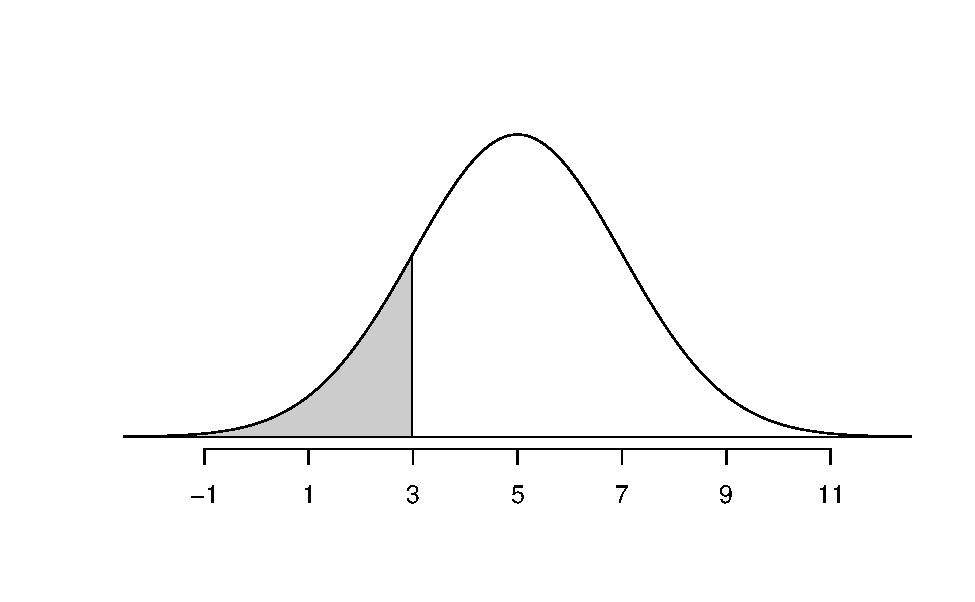
\includegraphics[width=0.6\linewidth]{07-RG-1cat_theory_files/figure-latex/normgt3-1} 

}

\end{figure}

Changing \texttt{L} to \texttt{U} will shade the area \emph{above} \texttt{x}.

Example: \texttt{normTail(m\ =\ 5,\ s\ =\ 2,\ U\ =\ 3)} plots a N(5,2) distribution with the area above 3 shaded.

\hypertarget{calculating-normal-percentiles}{%
\paragraph*{Calculating normal percentiles}\label{calculating-normal-percentiles}}
\addcontentsline{toc}{paragraph}{Calculating normal percentiles}

When using the \texttt{qnorm()} R function, you will need to enter values for the arguments \texttt{mean}, \texttt{sd}, and \texttt{p} to match the question.

\begin{Shaded}
\begin{Highlighting}[]
\FunctionTok{qnorm}\NormalTok{(}\AttributeTok{mean =}\NormalTok{ mu, }\AttributeTok{sd =}\NormalTok{ sigma, }\AttributeTok{p =}\NormalTok{ x, }\AttributeTok{lower.tail =} \ConstantTok{TRUE}\NormalTok{)}
\end{Highlighting}
\end{Shaded}

This function will return the value on the N(\texttt{mu}, \texttt{sigma}) distribution which has \texttt{x} area of the distribution \emph{below} it.

Example: \texttt{qnorm(mean\ =\ 5,\ sd\ =\ 2,\ p\ =\ 0.159,\ lower.tail\ =\ TRUE)} will give us the value on a N(5,2) distribution which has 0.159 (15.9\%) of the distribution below it, which equals 3 (from the R output above).

Changing to \texttt{lower.tail\ =\ FALSE} will give the value which has \texttt{x} area of the distribution \emph{above} it.

We would recommend you work through each of the examples in Section 5.2.4 using R.

\hypertarget{section-14.3-theory-based-inferential-methods-for-pi}{%
\subsection*{\texorpdfstring{Section 14.3 (Theory-based inferential methods for \(\pi\))}{Section 14.3 (Theory-based inferential methods for \textbackslash pi)}}\label{section-14.3-theory-based-inferential-methods-for-pi}}
\addcontentsline{toc}{subsection}{Section 14.3 (Theory-based inferential methods for \(\pi\))}

\setstretch{1}

\textbf{Videos}

\begin{itemize}
\tightlist
\item
  14.3TheoryTests
\item
  14.3TheoryIntervals
\end{itemize}

\setstretch{1.25}

\hypertarget{vocabulary-1}{%
\subsubsection*{Vocabulary}\label{vocabulary-1}}
\addcontentsline{toc}{subsubsection}{Vocabulary}

\hypertarget{reminders-from-previous-sections-1}{%
\subsubsection*{Reminders from previous sections}\label{reminders-from-previous-sections-1}}
\addcontentsline{toc}{subsubsection}{Reminders from previous sections}

\(n\) = sample size

\(\hat{p}\) = sample proportion

\(\pi\) = population proportion

General steps of a hypothesis test:

\begin{enumerate}
\def\labelenumi{\arabic{enumi}.}
\item
  Frame the research question in terms of hypotheses.
\item
  Collect and summarize data using a test statistic.
\item
  Assume the null hypothesis is true, and simulate or mathematically model a null distribution for the test statistic.
\item
  Compare the observed test statistic to the null distribution to calculate a p-value.
\item
  Make a conclusion based on the p-value and write the conclusion in context.
\end{enumerate}

Parameter: a value summarizing a variable(s) for a population.

Statistic: a value summarizing a variable(s) for a sample.

Sampling distribution: plot of statistics from 1000s of samples of the same size taken from the same population.

Standard deviation of a statistic: the variability of statistics from 1000s of samples; how far, on average, each statistic is from the true value of the parameter.

Standard error of a statistic: estimated standard deviation of a statistic.

Hypothesis test: a process to determine how strong the evidence of an effect is.

\rgi Also called a `significance test'.

Theory-based method: Develop a mathematical model for the sampling distribution of the statistic under the null hypothesis and use the model to calculate the probability of the observed sample statistic (or one more extreme) occurring.

Null hypothesis (\(H_0\)): the skeptical perspective; no difference; no change; no effect; random chance; what the researcher hopes to prove is \textbf{wrong}.

Alternative hypothesis (\(H_A\)): the new perspective; a difference/increase/decrease; an effect; not random chance; what the researcher hopes to prove is \textbf{correct}.

P-value: probability of seeing the observed sample data, or something more extreme, assuming the null hypothesis is true.

\(\implies\) Lower the p-value the stronger the evidence AGAINST the null hypothesis and FOR the alternative hypothesis.

Decision: a determination of whether to `reject' or `fail to reject' a null hypothesis based on a p-value and a pre-set level of significance.

Significance level (\(\alpha\)): a threshold used to determine if a p-value provides enough evidence to reject the null hypothesis or not.

\rgi Common levels of \(\alpha\) include 0.01, 0.05, and 0.10.

Statistically significant: results are considered statistically significant if the p-value is below the significance level.

Central Limit Theorem: For large sample sizes, the sampling distribution of a sample proportion (or mean) will be approximately normal (bell-shaped and symmetric).

Confidence interval: a process to determine how large an effect is; a range of plausible values for the parameter; also called `estimation'.

Margin of error: the value that is added to and subtracted from the sample statistic to create a confidence interval; half the width of a confidence interval.

\hypertarget{vocabulary-2}{%
\subsubsection*{Vocabulary}\label{vocabulary-2}}
\addcontentsline{toc}{subsubsection}{Vocabulary}

Null standard error:
\rgs

Standardized statistic:
\rgs

Confidence level:
\rgs

\hypertarget{notes-1}{%
\subsubsection*{Notes}\label{notes-1}}
\addcontentsline{toc}{subsubsection}{Notes}

Conditions for the Central Limit Theorem to apply (for the sampling distribution of \(\hat{p}\) to be approximately normal)

\rgi Independence:
\rgs

\rgi \rgi Checked by:
\rgs

\rgi Success-failure condition:
\rgs

\rgi \rgi Checked by:
\rgs

How can we determine the value of \(z^⋆\) to use as the multiplier in a confidence interval?
\rgs

\rgi In R, use \texttt{qnorm(mean\ =\ \_\_,\ sd\ =\ \_\_,\ p\ =\ \_\_)}.

Select one answer in each set of parentheses: The higher the confidence level, the (larger/smaller) the multiplier, meaning the confidence interval will be (wider/narrower).

If the success-failure condition for the Central Limit Theorem is not met, what is the appropriate method of analysis? Select one:
\rgi A. Theory-based approach
\rgi B. Simulation based approach.

\hypertarget{formulas-1}{%
\subsubsection*{Formulas}\label{formulas-1}}
\addcontentsline{toc}{subsubsection}{Formulas}

\(SD(\hat{p})\) =
\rgs

Null standard error of the sample proportion:

\(SE_0(\hat{p})\) =
\rgs

Standardized statistic (in this case, standardized sample proportion):

\(Z\) =
\rgs

Standard error of the sample proportion when we do not assume the null hypothesis is true:

\(SE(\hat{p})\) =
\rgs

Theory-based confidence interval for a sample proportion:
\rgs

Margin of error of a confidence interval for a sample proportion:
\rgs

\hypertarget{example-payday-loans}{%
\subsubsection*{Example: Payday loans}\label{example-payday-loans}}
\addcontentsline{toc}{subsubsection}{Example: Payday loans}

\begin{enumerate}
\def\labelenumi{\arabic{enumi}.}
\item
  What is the parameter representing in the context of this problem? What notation would be used to represent this parameter?
  \rgs
  \rgs
\item
  Write the null and alternative hypotheses in words.
  \rgs
  \rgs
\item
  Write the null and alternative hypotheses in notation.
  \rgs
\item
  Are the conditions met to use theoretical methods to analyze these data? Show your calculations to justify your answer.
  \rgs
  \rgs
\item
  Calculate the null standard error of the sample proportion.
  \rgs
  \rgs
\item
  What is the sample statistic presented in this example? What notation would be used to represent this value?
  \rgs
\item
  Calculate the standardized sample proportion (standardized statistic).
  \rgs
  \rgs
\item
  How can we calculate a p-value from the normal distribution for this example?
  \rgs
  \rgs
\item
  What was the p-value of the test?
  \rgs
\item
  What conclusion should the researcher make?
  \rgs
  \rgs
\item
  Are the results in this example statistically significant? Justify your answer.
  \rgs
\item
  Calculate the standard error of the sample proportion when we do not assume the null hypothesis is true.
  \rgs
  \rgs
\item
  Calculate the margin of error for a 95\% confidence interval for \(\pi\) using 1.96 as the multiplier.
  \rgs
  \rgs
\item
  Calculate a 95\% confidence interval for \(\pi\) using your margin of error calculated above.
  \rgs
  \rgs
\item
  Interpret the 95\% confidence interval provided in the textbook.
  \rgs
  \rgs
\item
  Does the 95\% confidence interval support the same conclusion as the p-value from the hypothesis test? Justify your answer.
  \rgs
\end{enumerate}

\hypertarget{chapter-12-errors-power-and-practical-importance}{%
\subsection*{Chapter 12 (Errors, power, and practical importance)}\label{chapter-12-errors-power-and-practical-importance}}
\addcontentsline{toc}{subsection}{Chapter 12 (Errors, power, and practical importance)}

\setstretch{1}

\textbf{Videos}

\begin{itemize}
\tightlist
\item
  Chapter12
\end{itemize}

\setstretch{1.25}

\hypertarget{reminders-from-previous-sections-2}{%
\subsubsection*{Reminders from previous sections}\label{reminders-from-previous-sections-2}}
\addcontentsline{toc}{subsubsection}{Reminders from previous sections}

Significance level (\(\alpha\)): a threshold used to determine if a p-value provides enough evidence to reject the null hypothesis or not.

\rgi Common levels of \(\alpha\) include 0.01, 0.05, and 0.10.

Statistically significant: results are considered statistically significant if the p-value is below the significance level.

\hypertarget{vocabulary-3}{%
\subsubsection*{Vocabulary}\label{vocabulary-3}}
\addcontentsline{toc}{subsubsection}{Vocabulary}

Decision:

\rgs

\begin{itemize}
\item
  If the p-value is small (less than or equal to the significance level), the decision will be to \_\_\_\_\_\_\_\_\_\_ the null hypothesis.
\item
  If the p-value is large (greater than the significance level), the decision will be to \_\_\_\_\_\_\_\_\_\_ the null hypothesis.
\end{itemize}

Type 1 error:
\rgs

Type 2 error:
\rgs

Confirmation bias:
\rgs

One-sided hypothesis tests:
\rgs

Two-sided hypothesis tests:
\rgs

Power:
\rgs

Practical importance:
\rgs

\hypertarget{notes-2}{%
\subsubsection*{Notes}\label{notes-2}}
\addcontentsline{toc}{subsubsection}{Notes}

Fill in the following table with whether the decision was correct or not, and if not, what type of error was made.

\begin{center}
\begin{tabular}{|p{2in}|p{2in}|p{2in}|}
\hline
 & \multicolumn{2}{|c|}{\textbf{Test conclusion (based on data)}} \\ \hline
 \textbf{Truth (unknown)} & Reject null hyp. & Fail to reject null hyp. \\ \hline
 $H_0$ is true && \\ 
   & & \\ 
   & & \\ \hline
 $H_A$ is true ($H_0$ is false)  && \\ 
   & & \\ 
   & & \\ \hline
\end{tabular}
\end{center}

\rgs

How are the significance level and type I error rate related?
\rgs

How are the significance level and type II error rate related?
\rgs

Explain the differences between a one-sided and two-sided hypothesis test.
\vspace{1mm}

\rgi How will the research questions differ?
\rgs

\rgi How will the notation in the alternative hypothesis differ?
\rgs

\rgi How does the p-value calculation differ?
\rgs

How does the p-value in a two-sided test compare to the p-value in a one-sided test?
\rgs

Should the default in research be a one-sided or two-sided hypothesis test? Explain why.
\rgs
\rgs

After collecting data, a researcher decides to change from a two-sided test to a one-sided test. Why is this a bad idea?

\begin{enumerate}
\def\labelenumi{\arabic{enumi}.}
\item
  It \_\_\_\_\_\_\_\_\_\_\_\_ (increases/decreases) the chance of a type I error.
\item
  This can result in \_\_\_\_\_\_\_\_\_\_\_\_\_\_\_\_\_\_\_\_\_\_\_\_.
  \rgs
\end{enumerate}

How are power and type I error rate related?
\rgs

How are power and type II error rate related?
\rgs

How can we increase the power of a test?

\begin{enumerate}
\def\labelenumi{\arabic{enumi}.}
\item
  \_\_\_\_\_\_\_\_ (Increase/Decrease) the significance level
  \rgs
\item
  \_\_\_\_\_\_\_\_ (Increase/Decrease) the sample size
  \rgs
\item
  Change from a \_\_\_ (one/two)-sided to a \_\_\_ (one/two)-sided test
  \rgs
\item
  Have a \_\_\_\_\_\_\_\_ (larger/smaller) standard deviation of the statistic
  \rgs
\item
  Have the alternative parameter value \_\_\_\_\_\_\_ (closer/farther) from the null value
  \rgs
\end{enumerate}

Results are likely to be statistically significant (but may not be practically important) if the sample size is \_\_\_\_\_\_\_\_\_\_(large/small).
\rgs

Results are unlikely to be statistically significant (but may be practically important) if the sample size is \_\_\_\_\_\_\_\_\_\_(large/small).
\rgs

\hypertarget{examples}{%
\subsubsection*{Examples:}\label{examples}}
\addcontentsline{toc}{subsubsection}{Examples:}

\begin{enumerate}
\def\labelenumi{\arabic{enumi}.}
\tightlist
\item
  In the Martian Alphabet study section 9.1 of the textbook,
\end{enumerate}

\rgi a. What was the p-value of the test?
\rgs

\rgi b. At the 5\% significance level, what decision would you make?
\rgs

\rgi c.~What type of error might have occurred in these data?
\rgs

\rgi d.~Interpret that error in the context of the problem.
\rgs
\rgs

\begin{enumerate}
\def\labelenumi{\arabic{enumi}.}
\setcounter{enumi}{1}
\tightlist
\item
  In the Medical Consultant study in section 10.1 of the textbook,
\end{enumerate}

\rgi a. What was the p-value of the test?
\rgs

\rgi b. At the 5\% significance level, what decision would you make?
\rgs

\rgi c.~What type of error might have occurred in these data?
\rgs

\rgi d.~Interpret that error in the context of the problem.
\rgs
\rgs

\begin{enumerate}
\def\labelenumi{\arabic{enumi}.}
\setcounter{enumi}{2}
\tightlist
\item
  In the Payday Loans study section 14.3 of the textbook,
\end{enumerate}

\rgi a. What was the p-value of the test?
\rgs

\rgi b. At the 5\% significance level, what decision would you make?
\rgs

\rgi c.~What type of error might have occurred in these data?
\rgs

\rgi d.~Interpret that error in the context of the problem.
\rgs

\newpage

\hypertarget{activity-7a-helper-hinderer-simulation-based-confidence-interval}{%
\section{Activity 7A: Helper-Hinderer --- Simulation-based Confidence Interval}\label{activity-7a-helper-hinderer-simulation-based-confidence-interval}}

\setstretch{1}

\hypertarget{learning-outcomes}{%
\subsection{Learning outcomes}\label{learning-outcomes}}

\begin{itemize}
\item
  Use bootstrapping to find a confidence interval for a single proportion.
\item
  Interpret a confidence interval for a single proportion.
\end{itemize}

\hypertarget{terminology-review}{%
\subsection{Terminology review}\label{terminology-review}}

In today's activity, we will introduce simulation-based confidence intervals for a single proportion. Some terms covered in this activity are:

\begin{itemize}
\item
  Parameter of interest
\item
  Bootstrapping
\item
  Confidence interval
\end{itemize}

To review these concepts, see Chapters 10 \& 14 in your textbook.

\hypertarget{helper-hinderer}{%
\subsection{Helper-Hinderer}\label{helper-hinderer}}

In the last class, we found very strong evidence that the true proportion of infants who will choose the helper character is greater than 0.5. But what \emph{is} the true proportion of infants who will choose the helper character? We will use this same study to estimate this parameter of interest by creating a confidence interval.

As a reminder: A study by Hamblin, Wynn, and Bloom reported in Nature (Hamblin, Wynn, and Bloom 2007) was intended to check young kids' feelings about helpful and non-helpful behavior. Non-verbal infants ages 6 to 10 months were shown short videos with different shapes either helping or hindering the climber. Researchers were hoping to assess: Are infants more likely to preferentially choose the helper toy over the hinderer toy? In the study, of the 16 infants age 6 to 10 months, 14 chose the \emph{helper} toy and 2 chose the \emph{hinderer} toy.

A \textbf{point estimate} (our observed statistic) provides a single plausible value for a parameter. However, a point estimate is rarely perfect; usually there is some error in the estimate. In addition to supplying a point estimate of a parameter, a next logical step would be to provide a plausible \emph{range} of values for the parameter. This plausible range of values for the population parameter is called an \textbf{interval estimate} or \textbf{confidence interval}.

\hypertarget{activity-intro}{%
\subsubsection*{Activity intro}\label{activity-intro}}
\addcontentsline{toc}{subsubsection}{Activity intro}

\begin{enumerate}
\def\labelenumi{\arabic{enumi}.}
\tightlist
\item
  What is the value of the point estimate?
\end{enumerate}

\vspace{0.3in}

\begin{enumerate}
\def\labelenumi{\arabic{enumi}.}
\setcounter{enumi}{1}
\tightlist
\item
  If we took another random sample of 16 infants, would we get the exact same point estimate? Explain why or why not.
\end{enumerate}

\vspace{0.5in}

In today's activity, we will use bootstrapping, sampling with replacement from the original sample, to find a 95\% confidence interval for \(\pi\), the parameter of interest.

\hypertarget{use-statistical-analysis-methods-to-draw-inferences-from-the-data}{%
\subsubsection*{Use statistical analysis methods to draw inferences from the data}\label{use-statistical-analysis-methods-to-draw-inferences-from-the-data}}
\addcontentsline{toc}{subsubsection}{Use statistical analysis methods to draw inferences from the data}

To use the computer simulation to create a bootstrap distribution, we will need to enter the

\begin{itemize}
\tightlist
\item
  ``sample size'' (the number of observational units or cases in the sample),
\item
  ``number of successes'' (the number of cases that choose the helper character),
\item
  ``number of repetitions'' (the number of samples to be generated), and
\item
  the ``confidence level'' (which level of confidence are we using to create the confidence interval).
\end{itemize}

\begin{enumerate}
\def\labelenumi{\arabic{enumi}.}
\setcounter{enumi}{2}
\tightlist
\item
  What values should be entered for each of the following into the simulation to create the bootstrap distribution of sample proportions to find a 95\% confidence interval?
  \vspace{1mm}
\end{enumerate}

\begin{itemize}
\tightlist
\item
  Sample size:
\end{itemize}

\vspace{.1in}

\begin{itemize}
\tightlist
\item
  Number of successes:
\end{itemize}

\vspace{.1in}

\begin{itemize}
\tightlist
\item
  Number of repetitions:
\end{itemize}

\vspace{.1in}

\begin{itemize}
\tightlist
\item
  Confidence level (as a decimal):
\end{itemize}

\vspace{.1in}

We will use the \texttt{one\_proportion\_bootstrap\_CI()} function in R (in the \texttt{catstats} package) to simulate the bootstrap distribution of sample proportions and calculate a confidence interval. Using the provided R script file, fill in the values/words for each \texttt{xx} with your answers from question 3 in the one proportion bootstrap confidence interval (CI) code to create a bootstrap distribution with 1000 simulations. Then highlight and run lines 1--9.

\begin{Shaded}
\begin{Highlighting}[]
\FunctionTok{one\_proportion\_bootstrap\_CI}\NormalTok{(}\AttributeTok{sample\_size =}\NormalTok{ xx, }\CommentTok{\# Sample size}
                    \AttributeTok{number\_successes =}\NormalTok{ xx, }\CommentTok{\# Observed number of successes}
                    \AttributeTok{number\_repetitions =} \DecValTok{1000}\NormalTok{, }\CommentTok{\# Number of bootstrap samples to use}
                    \AttributeTok{confidence\_level =} \FloatTok{0.95}\NormalTok{) }\CommentTok{\# Confidence level as a decimal}
\end{Highlighting}
\end{Shaded}

\begin{enumerate}
\def\labelenumi{\arabic{enumi}.}
\setcounter{enumi}{3}
\tightlist
\item
  Sketch the bootstrap distribution created below.
\end{enumerate}

\vspace{1.8in}

\begin{enumerate}
\def\labelenumi{\arabic{enumi}.}
\setcounter{enumi}{4}
\item
  What is the value at the center of this bootstrap distribution? Why does this make sense?
  \vspace{.8in}
\item
  Explain why the two vertical lines are at the 2.5th percentile and the 97.5th percentile.
\end{enumerate}

\vspace{.7in}

\begin{enumerate}
\def\labelenumi{\arabic{enumi}.}
\setcounter{enumi}{6}
\tightlist
\item
  Report the 95\% bootstrapped confidence interval for \(\pi\). Use interval notation: (lower value, upper value).
\end{enumerate}

\vspace{0.2in}

\begin{enumerate}
\def\labelenumi{\arabic{enumi}.}
\setcounter{enumi}{7}
\tightlist
\item
  Interpret the 95\% confidence interval in context.
\end{enumerate}

\vspace{.7in}

\hypertarget{communicate-the-results-and-answer-the-research-question}{%
\subsubsection*{Communicate the results and answer the research question}\label{communicate-the-results-and-answer-the-research-question}}
\addcontentsline{toc}{subsubsection}{Communicate the results and answer the research question}

\begin{enumerate}
\def\labelenumi{\arabic{enumi}.}
\setcounter{enumi}{8}
\tightlist
\item
  Is the value 0.5 (the null value) in the 95\% confidence interval?
\end{enumerate}

\vspace{.2in}

\rgi Explain how this indicates that the p-value will provide similar evidence against the null hypothesis.

\vspace{0.5in}

\hypertarget{effect-of-confidence-level}{%
\subsubsection*{Effect of confidence level}\label{effect-of-confidence-level}}
\addcontentsline{toc}{subsubsection}{Effect of confidence level}

\begin{enumerate}
\def\labelenumi{\arabic{enumi}.}
\setcounter{enumi}{9}
\tightlist
\item
  Suppose instead of finding a 95\% confidence interval, we found a 90\% confidence interval. Would you expect the 90\% confidence interval to be narrower or wider? Explain your answer.
\end{enumerate}

\vspace{0.4in}

\newpage

\begin{enumerate}
\def\labelenumi{\arabic{enumi}.}
\setcounter{enumi}{10}
\tightlist
\item
  The following R code produced the bootstrap distribution with 1000 simulations that follows. Circle the value that changed in the code.
\end{enumerate}

\begin{Shaded}
\begin{Highlighting}[]
\FunctionTok{one\_proportion\_bootstrap\_CI}\NormalTok{(}\AttributeTok{sample\_size =} \DecValTok{16}\NormalTok{, }\CommentTok{\# Sample size}
                    \AttributeTok{number\_successes =} \DecValTok{14}\NormalTok{, }\CommentTok{\# Observed number of successes}
                    \AttributeTok{number\_repetitions =} \DecValTok{1000}\NormalTok{, }\CommentTok{\# Number of bootstrap samples to use}
                    \AttributeTok{confidence\_level =} \FloatTok{0.90}\NormalTok{) }\CommentTok{\# Confidence level as a decimal}
\end{Highlighting}
\end{Shaded}

\begin{center}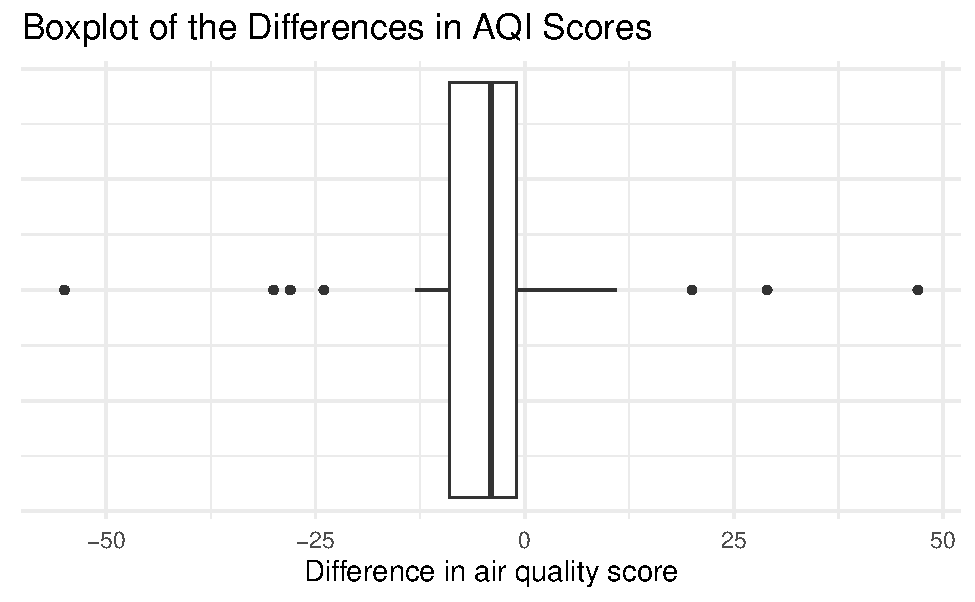
\includegraphics[width=0.7\linewidth]{07-A09-inference-1cat_CI-simulation_files/figure-latex/unnamed-chunk-2-1} \end{center}

\begin{enumerate}
\def\labelenumi{\arabic{enumi}.}
\setcounter{enumi}{11}
\tightlist
\item
  Report both the 95\% confidence interval (question 7) and the 90\% confidence interval (question 11). Is the 90\% confidence interval narrower or wider than the 95\% confidence interval?
\end{enumerate}

\vspace{0.5in}

\hypertarget{what-does-confidence-mean}{%
\subsection*{\texorpdfstring{What does \emph{confidence} mean?}{What does confidence mean?}}\label{what-does-confidence-mean}}
\addcontentsline{toc}{subsection}{What does \emph{confidence} mean?}

In the interpretation of a 95\% confidence interval, we say that we are 95\% confident that the parameter is within the confidence interval. Why are we able to make that claim? What does it mean to say ``we are 95\% confident''?

For this part of the activity we will assume that the the true proportion of infants who choose the helper is 0.65. \emph{Note: we are making assumptions about the population here. This is not based on our calculated data, but we will use this applet to better understand what happens when we take many, many samples from this believed population.}

\begin{enumerate}
\def\labelenumi{\arabic{enumi}.}
\setcounter{enumi}{12}
\tightlist
\item
  Go to this website, \url{http://www.rossmanchance.com/ISIapplets.html} and choose `Simulating Confidence Intervals'. In the input on the left-hand side of the screen enter 0.65 for \(\pi\) (the true value), 16 for \(n\), and 100 for `Number of intervals'. Click `sample'.
  \vspace{1mm}
\end{enumerate}

\begin{enumerate}
\def\labelenumi{\alph{enumi}.}
\item
  In the graph on the bottom right, click on a green dot. Write down the confidence interval for this sample given on the graph on the left. Does this confidence interval contain the true value of 0.65?
  \vspace{0.5in}
\item
  Now click on a red dot. Write down the confidence interval for this sample. Does this confidence interval contain the true value of 0.65?
  \vspace{0.5in}
\item
  How many intervals out of 100 contain \(\pi\), the true value of 0.65? \emph{Hint}: This is given to the left of the graph of green and red intervals.
  \vspace{0.5in}
\end{enumerate}

\begin{enumerate}
\def\labelenumi{\arabic{enumi}.}
\setcounter{enumi}{13}
\tightlist
\item
  Click on `sample' nine more times. Write down the `Running Total' for the proportion of intervals that contain \(\pi\).
\end{enumerate}

\vspace{0.5in}

\begin{enumerate}
\def\labelenumi{\arabic{enumi}.}
\setcounter{enumi}{14}
\tightlist
\item
  Interpret the level of confidence in context of the problem. \emph{Hint}: What proportion of samples would we expect to give a confidence interval that contains the parameter of interest?
\end{enumerate}

\vspace{0.8in}

\hypertarget{take-home-messages}{%
\subsection{Take-home messages}\label{take-home-messages}}

\begin{enumerate}
\def\labelenumi{\arabic{enumi}.}
\item
  The goal in a hypothesis test is to assess the strength of evidence for an effect, while the goal in creating a confidence interval is to determine how large the effect is. A \textbf{confidence interval} is a range of \emph{plausible} values for the parameter of interest.
\item
  A confidence interval is built around the point estimate or observed calculated statistic from the sample. This means that the sample statistic is always the center of the confidence interval. A confidence interval includes a measure of sample to sample variability represented by the \textbf{margin of error}.
\item
  In simulation-based methods (bootstrapping), a simulated distribution of possible sample statistics is created showing the possible sample-to-sample variability. Then we find the middle \(X\) percent of the distribution around the sample statistic using the percentile method to give the range of values for the confidence interval. This shows us that we are \(X\)\% confident that the parameter is within this range, where \(X\) represents the level of confidence.
\item
  When the null value is within the confidence interval, it is a plausible value for the parameter of interest; thus, we would find a larger p-value for a hypothesis test of that null value. Conversely, if the null value is NOT within the confidence interval, we would find a small p-value for the hypothesis test and strong evidence against this null hypothesis.
\item
  To create one simulated sample on the bootstrap distribution for a sample proportion, label \(n\) cards with the original responses. Draw with replacement \(n\) times. Calculate and plot the resampled proportion of successes.
\item
  If repeat samples of the same size are selected from the population, approximately 95\% of samples will create a 95\% confidence interval that contains the parameter of interest.
\end{enumerate}

\newpage

\hypertarget{additional-notes}{%
\subsection{Additional notes}\label{additional-notes}}

Use this space to summarize your thoughts and take additional notes on today's activity and material covered.

\newpage

\hypertarget{activity-7b-handedness-of-male-boxers-theory-based-methods}{%
\section{Activity 7B: Handedness of Male Boxers --- Theory-based Methods}\label{activity-7b-handedness-of-male-boxers-theory-based-methods}}

\setstretch{1}

\hypertarget{learning-objectives}{%
\subsection{Learning objectives}\label{learning-objectives}}

\begin{itemize}
\item
  Describe and perform a theory-based hypothesis test for a single proportion.
\item
  Check the appropriate conditions to use a theory-based methods.
\item
  Calculate and interpret the standardized sample proportion.
\item
  Interpret and evaluate a p-value for a theory-based hypothesis test for a single proportion.
\item
  Use the normal distribution to find the p-value.
\item
  Calculate a theory-based confidence interval for a single proportion.
\item
  Interpret a confidence interval for a single proportion.
\item
  Use the normal distribution to find the multiplier needed for a confidence interval
\end{itemize}

\hypertarget{terminology-review-1}{%
\subsection{Terminology review}\label{terminology-review-1}}

In this activity, we will introduce theory-based hypothesis tests and confidence intervals for a single proportion. Some terms covered in this activity are:

\begin{itemize}
\item
  Parameter of interest
\item
  Standardized Statistic
\item
  Normal distribution
\item
  p-value
\item
  Multiplier
\item
  Normal distribution
\end{itemize}

To review these concepts, see Chapters 11 \& 14 in your textbook.

Activities 6A, 6B, and 7A covered simulation-based methods for hypothesis tests involving a single categorical variable. This activity covers theory-based methods for testing a single categorical variable.

\hypertarget{handedness-of-male-boxers}{%
\subsection{Handedness of male boxers}\label{handedness-of-male-boxers}}

Left-handedness is a trait that is found in about 10\% of the general population. Past studies have shown that left-handed men are over-represented among professional boxers (Richardson and Gilman 2019). The fighting claim states that left-handed men have an advantage in competition. In this random sample of 500 male professional boxers, we want to see if there is an over-prevalence of left-handed fighters. In the sample of 500 male boxers, 81 were left-handed.

\begin{Shaded}
\begin{Highlighting}[]
 \CommentTok{\# Read in data set}
\NormalTok{boxers }\OtherTok{\textless{}{-}} \FunctionTok{read.csv}\NormalTok{(}\StringTok{"https://math.montana.edu/courses/s216/data/Male\_boxers\_sample.csv"}\NormalTok{)}
\NormalTok{boxers }\SpecialCharTok{\%\textgreater{}\%} \FunctionTok{count}\NormalTok{(Stance)  }\CommentTok{\# Count number in each Stance category}
\end{Highlighting}
\end{Shaded}

\begin{verbatim}
#>         Stance   n
#> 1  left-handed  81
#> 2 right-handed 419
\end{verbatim}

\hypertarget{review-of-summary-statistics}{%
\subsection*{Review of summary statistics}\label{review-of-summary-statistics}}
\addcontentsline{toc}{subsection}{Review of summary statistics}

\begin{enumerate}
\def\labelenumi{\arabic{enumi}.}
\tightlist
\item
  Write out the parameter of interest for this study.
\end{enumerate}

\vspace{0.6in}

\begin{enumerate}
\def\labelenumi{\arabic{enumi}.}
\setcounter{enumi}{1}
\item
  Write out the null hypothesis in words.
  \vspace{0.6in}
\item
  Write out the alternative hypothesis in notation.
  \vspace{0.3in}
\item
  Give the value of the summary statistic (sample proportion) for this study. Use proper notation.
\end{enumerate}

\vspace{0.3in}

\hypertarget{theory-based-methods}{%
\subsection*{Theory-based methods}\label{theory-based-methods}}
\addcontentsline{toc}{subsection}{Theory-based methods}

The sampling distribution of a single proportion --- how that proportion varies from sample to sample --- can be mathematically modeled using the normal distribution if certain conditions are met.

Conditions for the sampling distribution of \(\hat{p}\) to follow an approximate normal distribution:

\begin{itemize}
\item
  \textbf{Independence}: The sample's observations are independent, e.g., are from a simple random sample. (\emph{Remember}: This also must be true to use simulation methods!)
\item
  \textbf{Success-failure condition}: We \emph{expect} to see at least 10 successes and 10 failures in the sample, \(n\hat{p}≥10\) and \(n(1-\hat{p})≥10\).
\end{itemize}

\begin{enumerate}
\def\labelenumi{\arabic{enumi}.}
\setcounter{enumi}{4}
\tightlist
\item
  Verify that the independence condition is satisfied.
\end{enumerate}

\vspace{0.8in}

\begin{enumerate}
\def\labelenumi{\arabic{enumi}.}
\setcounter{enumi}{5}
\tightlist
\item
  Is the success-failure condition met to model the data with the normal distribution? Show your work to support your answer.
\end{enumerate}

\vspace{1in}
\newpage

To calculate the standardized statistic we use the general formula

\[
Z = \frac{\text{point estimate} - \text{null value}}{SE_0(\text{point estimate})}.
\]
For a single categorical variable the standardized sample proportion is calculated using

\[
Z = \frac{\hat{p} - \pi_0}{SE_0(\hat{p})},
\]
where the standard error is calculated using the null value:

\[SE_0(\hat{p})=\sqrt{\frac{\pi_0(1-\pi_0)}{n}}\].

The standard error of the sample proportion measures the variability of possible sample proportions from the actual proportion. In other words, how far each possible sample proportion is from the actual proportion on average. For this study, the null standard error of the sample proportion is calculated using the null value, 0.1.

\[SE_0(\hat{p})=\sqrt{\frac{0.1(1-0.1)}{500}} = 0.013\].

\begin{enumerate}
\def\labelenumi{\arabic{enumi}.}
\setcounter{enumi}{6}
\tightlist
\item
  Interpret the null standard error of the sample proportion in context of the problem.
\end{enumerate}

\vspace{0.5in}

\begin{enumerate}
\def\labelenumi{\arabic{enumi}.}
\setcounter{enumi}{7}
\tightlist
\item
  Label the standard normal distribution (figure 7.1) with the null value as the center value (below the value of zero). Label the tick marks to the right of the null value by adding 1 standard error to the null value to represent 1 standard error, 2 standard errors, and 3 standard errors from the null. Repeat this process to the left of the null value by subtracting 1 standard error for each tick mark.
\end{enumerate}

\vspace{2mm}

\begin{figure}

{\centering 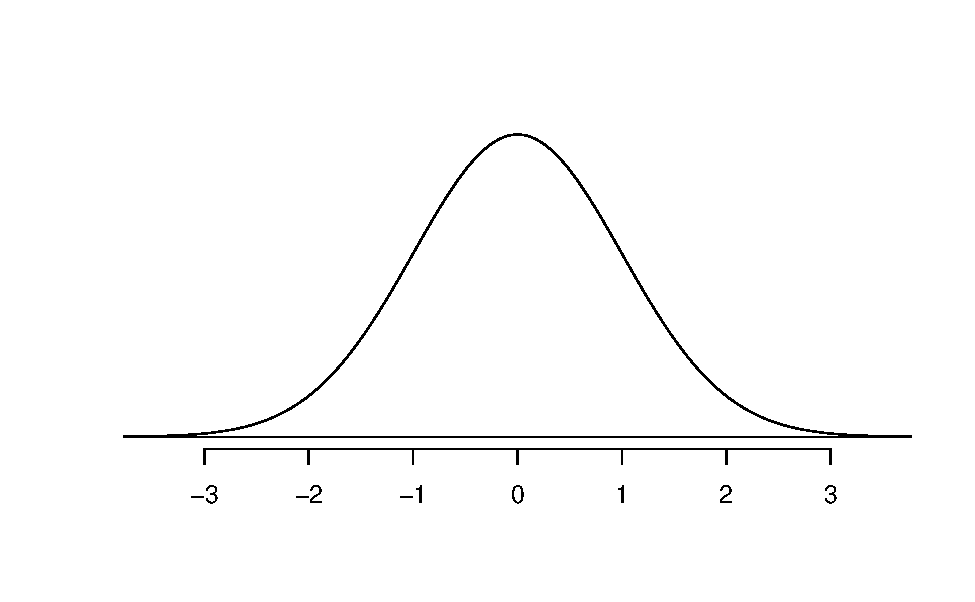
\includegraphics[width=0.5\linewidth]{07-A10-inference-1cat-theory_files/figure-latex/Normalcurve-1} 

}

\caption{Standard Normal Distribution}\label{fig:Normalcurve}
\end{figure}

\newpage

\begin{enumerate}
\def\labelenumi{\arabic{enumi}.}
\setcounter{enumi}{8}
\tightlist
\item
  Using the null standard error of the sample proportion, calculate the standardized sample proportion (Z). Mark this value on the standard normal distribution above.
\end{enumerate}

\vspace{0.6in}

The standardized statistic is used as a ruler to measure how far the sample statistic is from the null value. Essentially, we are converting the sample proportion into a measure of standard errors to compare to the standard normal distribution.

The standardized statistic measures the \emph{number of standard errors the sample statistic is from the null value}.

\begin{enumerate}
\def\labelenumi{\arabic{enumi}.}
\setcounter{enumi}{9}
\tightlist
\item
  Interpret the standardized sample proportion from question 9 in context of the problem.
\end{enumerate}

\vspace{.8in}

We will use the \texttt{pnorm()} function in R to find the p-value. Use the provided R script file and enter the value of the standardized statistic calculated in question 8 at \texttt{xx} in line 7; highlight and run lines 7--9. Notice that in line 9 it says \texttt{lower.tail\ =\ FALSE}. R will calculate the p-value \emph{greater} than the value of the standardized statistic.

Notes:

\begin{itemize}
\tightlist
\item
  Use \texttt{lower.tail\ =\ TRUE} when doing a left-sided test.
\item
  Use \texttt{lower.tail\ =\ FALSE} when doing a right-sided test.
\item
  To find a two-sided p-value, use a left-sided test for negative Z or a right-sided test for positive Z, then multiply the value found by 2 to get the p-value.
\end{itemize}

\begin{Shaded}
\begin{Highlighting}[]
\FunctionTok{pnorm}\NormalTok{(xx, }\CommentTok{\# Enter value of standardized statistic}
      \AttributeTok{m=}\DecValTok{0}\NormalTok{, }\AttributeTok{s=}\DecValTok{1}\NormalTok{, }\CommentTok{\# Using the standard normal mean = 0, sd = 1}
      \AttributeTok{lower.tail=}\ConstantTok{FALSE}\NormalTok{) }\CommentTok{\# Gives a p{-}value greater than the standardized statistic}
\end{Highlighting}
\end{Shaded}

\begin{enumerate}
\def\labelenumi{\arabic{enumi}.}
\setcounter{enumi}{10}
\tightlist
\item
  Report the p-value obtained from the R output.
  \vspace{0.3in}
\end{enumerate}

\newpage

\hypertarget{theory-based-confidence-interval}{%
\subsubsection*{Theory-based confidence interval}\label{theory-based-confidence-interval}}
\addcontentsline{toc}{subsubsection}{Theory-based confidence interval}

To calculate a theory-based 95\% confidence interval for \(\pi\), we will first find the \textbf{standard error} of \(\hat{p}\) by plugging in the value of \(\hat{p}\) for \(\pi\) in \(SD(\hat{p})\):

\[SE(\hat{p}) = \sqrt{\frac{\hat{p}(1-\hat{p})}{n}}.\]
Note that we do not include a ``0'' subscript, since we are not assuming a null hypothesis.

\begin{enumerate}
\def\labelenumi{\arabic{enumi}.}
\setcounter{enumi}{11}
\tightlist
\item
  Calculate the standard error of the sample proportion to find a 95\% confidence interval.
\end{enumerate}

\vspace{0.5in}

To find the confidence interval, we will add and subtract the \textbf{margin of error} to the point estimate:

\[\text{point estimate}\pm\text{margin of error}\]
\[\hat{p}\pm z^* \times SE(\hat{p})\]
\[ME = z^* \times SE(\hat{p})\]

The \(z^*\) multiplier is the percentile of a standard normal distribution that corresponds to our confidence level. If our confidence level is 95\%, we find the Z values that encompass the middle 95\% of the standard normal distribution. If 95\% of the standard normal distribution should be in the middle, that leaves 5\% in the tails, or 2.5\% in each tail.

\begin{enumerate}
\def\labelenumi{\arabic{enumi}.}
\setcounter{enumi}{12}
\tightlist
\item
  Fill in the normal distribution shown in figure 7.2 to show how R found the \(z^*\) multiplier.
\end{enumerate}

\begin{figure}

{\centering 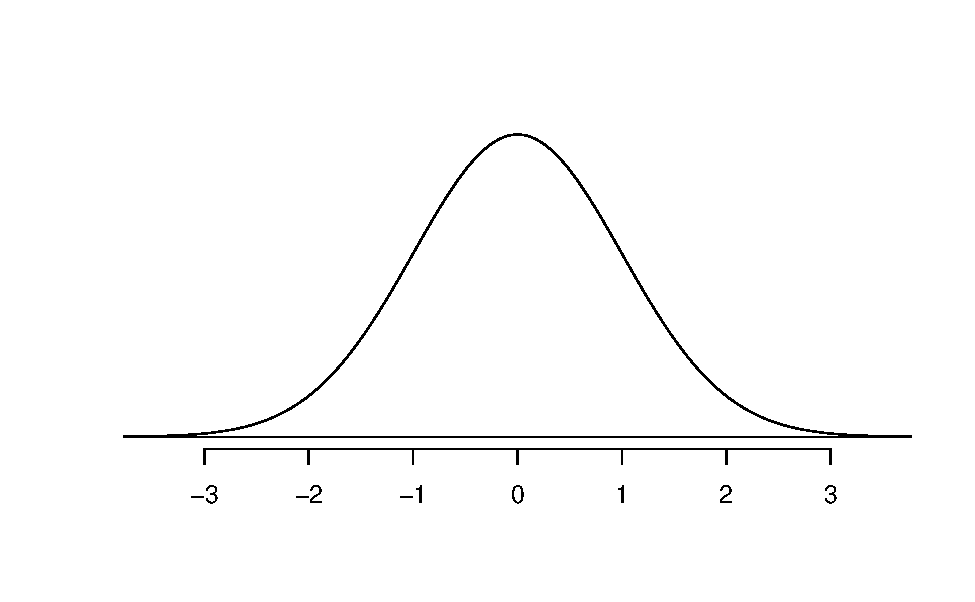
\includegraphics[width=0.5\linewidth]{07-A10-inference-1cat-theory_files/figure-latex/StandardNormal-1} 

}

\caption{Standard Normal Distribution}\label{fig:StandardNormal}
\end{figure}

\newpage

The \texttt{qnorm()} function in R will tell us the \(z^*\) value for the desired percentile (in this case, 95\% + 2.5\% = 97.5\% percentile). Enter the value of 0.975 for xx in the provided R script file. This will give the value of the multiplier for a 95\% confidence interval.

\begin{Shaded}
\begin{Highlighting}[]
\FunctionTok{qnorm}\NormalTok{(xx) }\CommentTok{\# Multiplier for 95\% confidence interval}
\end{Highlighting}
\end{Shaded}

\begin{enumerate}
\def\labelenumi{\arabic{enumi}.}
\setcounter{enumi}{13}
\item
  Report the value of the multiplier (\(z^*\)) found from the R code needed to calculate the 95\% confidence interval for the true proportion of male boxers that are left-handed?
  \vspace{0.3in}
\item
  Calculate the margin of error for the 95\% confidence interval.
  \vspace{0.8in}
\item
  Calculate the 95\% confidence interval for the parameter of interest.
  \vspace{0.5in}
\item
  Interpret the 95\% confidence interval in the context of the problem.
  \vspace{0.5in}
\item
  Write a conclusion to the study in context of the problem.
  \vspace{0.5in}
\item
  Is the null value, 0.1, contained in the 95\% confidence interval? Explain, based on the p-value from the earlier in activity, why you expected this to be true.
  \vspace{0.5in}
\end{enumerate}

\newpage

\hypertarget{take-home-messages-1}{%
\subsection{Take-home messages}\label{take-home-messages-1}}

\begin{enumerate}
\def\labelenumi{\arabic{enumi}.}
\item
  Both simulation and theory-based methods can be used to find a p-value for a hypothesis test. In order to use theory-based methods we need to check that both the independence and the success-failure conditions are met.
\item
  The standardized statistic measures how many standard errors the statistic is from the null value. The larger the standardized statistic the more evidence there is against the null hypothesis.
\item
  In theory-based methods, we add and subtract a margin of error to the sample statistic. The margin of error is calculated using a multiplier that corresponds to the level of confidence times the variability (standard error) of the statistic.
\item
  The confidence interval calculated using theory-based methods should be similar to the confidence interval found using simulation methods provided the success-failure condition is met.
\end{enumerate}

\hypertarget{additional-notes-1}{%
\subsection{Additional notes}\label{additional-notes-1}}

Use this space to summarize your thoughts and take additional notes on today's activity and material covered.

\newpage

\hypertarget{week-7-lab-errors-and-power}{%
\section{Week 7 Lab: Errors and Power}\label{week-7-lab-errors-and-power}}

\setstretch{1}

\hypertarget{learning-outcomes-1}{%
\subsection{Learning outcomes}\label{learning-outcomes-1}}

\begin{itemize}
\item
  Explain type 1 and type 2 errors in the context of a study.
\item
  Explain the power of a test in the context of a study.
\item
  Understand how changes in sample size, significance level, and the difference between the null value and the parameter value impact the power of a test.
\item
  Understand how significance level impacts the probability of a type 1 error.
\item
  Understand the relationship between the probability of a type 2 error and power.
\item
  Be able to distinguish between practical importance and statistical significance.
\end{itemize}

\hypertarget{terminology-review-2}{%
\subsection{Terminology review}\label{terminology-review-2}}

In this activity, we will examine the possible errors that can be made based on the decision in a hypothesis test as well as factors influencing the power of the test. Some terms covered in this activity are:

\begin{itemize}
\item
  Significance level
\item
  Type 1 error
\item
  Type 2 error
\item
  Power
\end{itemize}

To review these concepts, see Chapter 12 in the textbook.

\hypertarget{acl-recovery}{%
\subsection{ACL recovery}\label{acl-recovery}}

It is widely reported that the median recovery time for athletes who undergo surgery to repair a torn anterior cruciate ligament (ACL) is 8 months, indicating that 50\% of athletes return to their sport within 8 months after an ACL surgery. Suppose a local physical therapy company hopes to advertise that their rehabilitation program can increase this percentage.

\begin{enumerate}
\def\labelenumi{\arabic{enumi}.}
\item
  Write the parameter of interest (\(\pi\)) in words, in the context of this problem.
  \vspace{0.5in}
\item
  \textbf{Use proper notation to write the null and alternative hypothesis the company would need to test in order to check their advertisement claim.}
  \vspace{0.5in}
\end{enumerate}

After determining hypotheses and prior to collecting data, researchers should set a \textbf{significance level} for a hypothesis test. The significance level, represented by \(\alpha\) and most commonly 0.01, 0.05, or 0.10, is a cut-off for determining whether a p-value is small or not. The \emph{smaller} the p-value, the \emph{stronger} the evidence against the null hypothesis, so a p-value that is smaller than or equal to the significance level is strong enough evidence to \emph{reject the null hypothesis}. Similarly, the \emph{larger} the p-value, the \emph{weaker} the evidence against the null hypothesis, so a p-value that is larger than the significance level does not provide enough evidence against the null hypothesis and the researcher would \emph{fail to reject the null hypothesis}. Rejecting the null hypothesis or failing to reject the null hypothesis are the two \textbf{decisions} that can be made based on the data collected.

As you have already learned in this course, sample size of a study is extremely important. Often times, researchers will conduct what is called a power analysis to determine the appropriate sample size based on the goals of their research, including a desired \textbf{power} of their test. Power is the probability of correctly rejecting the null hypothesis, or the probability of the data providing strong evidence against the null hypothesis \emph{when the null hypothesis is false}.

The remainder of this lab will be spent investigating how different factors influence the power of a test, after which you will complete a power analysis for this physical therapy company.

\begin{itemize}
\item
  Navigate to \url{https://istats.shinyapps.io/power/}. \emph{Please note that this applet uses \(p_0\) to represent the null value rather than \(\pi_0\).}
\item
  Use the scale under ``Null Hypothesis value \(p_0\)'' to change the value to your null value from question 2.
\item
  Change the ``Alternative Hypothesis'' to the direction you wrote in question 2.
\item
  Leave all boxes un-checked. Do not change the scales under ``True value of \(p_0\)'', ``Sample size n'', or ``Type I Error \(\alpha\)''
\end{itemize}

The red distribution you see is the scaled-Normal distribution representing the null distribution for this hypothesis test, if the sample size was 50 and the significance level was 0.05. This means the red distribution is showing the probability of each possible sample proportion of athletes who returned to their sport within 8 months (\(\hat{p}\)) if we assume the null hypothesis is true.

\begin{enumerate}
\def\labelenumi{\arabic{enumi}.}
\setcounter{enumi}{2}
\item
  Based off this distribution and your alternative hypothesis, give one possible sample proportion which you think would lead to rejecting the null hypothesis. Explain how you decided on your value.
  \vspace{0.25in}
\item
  Check the box for ``Show Critical Value(s) and Rejection Region(s)''. You will now see a vertical line on the plot indicating the \emph{minimum} sample proportion which would lead to reject the null hypothesis. What is this value?\\
  \vspace{0.25in}
\item
  Notice that there are some sample proportions under the red line (when the null hypothesis is true) which would lead us to reject the null hypothesis. Give the range of sample proportions which would lead to rejecting the null hypothesis when the null hypothesis is true. What is the statistical name for this mistake?
  \vspace{0.4in}
\end{enumerate}

Check the ``Type I Error'' box under \textbf{Display}. This should verify (or correct) your answer to question 5! The area shaded in red represents the probability of making a \textbf{type 1 error} in our hypothesis test. Recall that a type 1 error is when we reject the null hypothesis even though the null hypothesis is true. To reject the null hypothesis, the p-value, which was found assuming the null hypothesis is true, must be less than or equal to the significance level. Therefore the significance level is the maximum probability of rejecting the null hypothesis when the null hypothesis is true, so the significance level IS the probability of making a type 1 error in a hypothesis test!

\begin{enumerate}
\def\labelenumi{\arabic{enumi}.}
\setcounter{enumi}{5}
\tightlist
\item
  \textbf{Based on the current applet settings, what percent of the null distribution is shaded red (what is the probability of making a type 1 error)?}
  \vspace{0.25in}
\end{enumerate}

Let's say this physical therapist company believes their program can get 70\% of athletes back to their sport within 8 months of an ACL surgery. In the applet, set the scale under ``True value of \(p\)'' to 0.7.

\begin{enumerate}
\def\labelenumi{\arabic{enumi}.}
\setcounter{enumi}{6}
\tightlist
\item
  Where is the blue distribution centered?
  \vspace{0.25in}
\end{enumerate}

The blue distribution that appears represents what the company believes, that 0.7 (not 0.5) is the true proportion of its clients who return to their sport within 8 months of ACL surgery. This blue distribution represents the idea that the \textbf{null hypothesis is false}.

\begin{enumerate}
\def\labelenumi{\arabic{enumi}.}
\setcounter{enumi}{7}
\tightlist
\item
  Consider the definition of power provided earlier in this lab. Do you believe the power of the test will be an area within the blue distribution or red distribution? How do you know? What about the probability of making a type 2 error?
  \vspace{1in}
\end{enumerate}

\begin{itemize}
\tightlist
\item
  Check the ``Type II Error'' and ``Power'' boxes under \textbf{Display}. This should verify (or correct) your answers to question 8! The area shaded in blue represents the probability of making a \textbf{type 2 error} in our hypothesis test (failing to reject the null hypothesis even though the null hypothesis is false). The area shaded in green represents the power of the test. Notice that the type 1 and type 2 errors rates and the power of the test are provided above the distribution.
\end{itemize}

\begin{enumerate}
\def\labelenumi{\arabic{enumi}.}
\setcounter{enumi}{8}
\tightlist
\item
  \textbf{Complete the following equation: Power + Type 2 Error Rate = . Explain why that equation makes sense.} \emph{Hint: Consider what power and type 2 error are conditional on.}
  \vspace{0.8in}
\end{enumerate}

Now let's investigate how changes in different factors influence the power of a test.

\begin{enumerate}
\def\labelenumi{\arabic{enumi}.}
\setcounter{enumi}{9}
\item
  Using the same sample size and significance level, change the ``True value of \(p\)'' to see the effect on Power.
  \setlength\tabcolsep{0.5cm}

  \begin{longtable}{|l|c|c|c|c|c|}
  \hline
  \textbf{True value of $p$}& 0.60 & 0.65 & 0.70 & 0.75 & 0.80 \\ \hline
  \textbf{Power} & & & & &  \\ \hline
  \end{longtable}
\item
  What is changing about the simulated distributions pictured as you change the ``True value of \(p\)''?
  \vspace{0.5in}
\item
  \textbf{How does increasing the distance between the null and believed true probability of success affect the power of the test?}
  \vspace{0.5in}
\item
  Using the same significance level, set the ``True value of \(p\)'' to 0.7 and change the sample size to see the effect on Power.
\end{enumerate}

\setlength\tabcolsep{0.6cm}
\begin{longtable}{|l|c|c|c|c|c|}
\hline
\textbf{Sample Size}& 20 & 40 & 50 & 60 & 80 \\ \hline
\textbf{Power} & & & & &  \\ \hline
\end{longtable}

\begin{enumerate}
\def\labelenumi{\arabic{enumi}.}
\setcounter{enumi}{13}
\item
  What is changing about the simulated distributions pictured as you change the sample size?
  \vspace{0.5in}
\item
  \textbf{How does increasing the sample size affect the power of the test?}
  \vspace{0.5in}
\item
  Using the same ``True value of \(p\)'', set the sample size to 50 and change the ``Type I Error \(\alpha\)'' to see the effect on Power.
\end{enumerate}

\setlength\tabcolsep{0.5cm}
\begin{longtable}{|l|c|c|c|c|c|}
\hline
\textbf{Type I Error $\alpha$}& 0.01 & 0.03 & 0.05 & 0.10 & 0.15 \\ \hline
\textbf{Power} & & & & &  \\ \hline
\end{longtable}

\begin{enumerate}
\def\labelenumi{\arabic{enumi}.}
\setcounter{enumi}{16}
\item
  What is changing about the simulated distributions pictured as you change the significance level?
  \vspace{0.5in}
\item
  \textbf{How does increasing the significance level affect the power of the test?}
  \vspace{0.5in}
\item
  \textbf{Complete the power analysis for this physical therapy company. The company believes 70\% of their patients will return to their sport within 8 months of ACL surgery. They want to limit the probability of a type 1 error to 10\% and the probability of a type 2 error to 15\%. What is the minimum number of athletes the company will need to collect data from in order to meet these goals? Use the applet to answer this question, then download your image created and upload the file to Gradescope.}
  \vspace{0.25in}
\end{enumerate}

\newpage

\begin{enumerate}
\def\labelenumi{\arabic{enumi}.}
\setcounter{enumi}{19}
\tightlist
\item
  Based on the goals outlined in question 19, which mistake below is the company more concerned about? In other words, which error were the researchers trying to minimize. Explain your answer.
\end{enumerate}

\begin{itemize}
\item
  Not being able to advertise their ACL recovery program is better than average when their program really is better.
\item
  Advertising their ACL recovery program is better even though it is not.
\end{itemize}

\vspace{0.8in}

\newpage

\hypertarget{inference-for-two-categorical-variables-simulation-based-methods}{%
\chapter{Inference for Two Categorical Variables: Simulation-based Methods}\label{inference-for-two-categorical-variables-simulation-based-methods}}

\hypertarget{week-8-reading-guide-hypothesis-testing-for-a-difference-in-proportions}{%
\section{Week 8 Reading Guide: Hypothesis Testing for a Difference in Proportions}\label{week-8-reading-guide-hypothesis-testing-for-a-difference-in-proportions}}

\hypertarget{section-15.1-randomization-test-for-h_0-pi_1---pi_2-0-and-section-15.2-bootstrap-confidence-interval-for-pi_1---pi_2}{%
\subsection*{\texorpdfstring{Section 15.1 (Randomization test for \(H_0: \pi_1 - \pi_2 = 0\)) and Section 15.2 (Bootstrap confidence interval for \(\pi_1 - \pi_2\))}{Section 15.1 (Randomization test for H\_0: \textbackslash pi\_1 - \textbackslash pi\_2 = 0) and Section 15.2 (Bootstrap confidence interval for \textbackslash pi\_1 - \textbackslash pi\_2)}}\label{section-15.1-randomization-test-for-h_0-pi_1---pi_2-0-and-section-15.2-bootstrap-confidence-interval-for-pi_1---pi_2}}
\addcontentsline{toc}{subsection}{Section 15.1 (Randomization test for \(H_0: \pi_1 - \pi_2 = 0\)) and Section 15.2 (Bootstrap confidence interval for \(\pi_1 - \pi_2\))}

You may skip example 15.1.4, which discussed hypothesis testing for \textbf{relative risk}. We will discuss relative risk in Week 14.

\textbf{Videos}

\begin{itemize}
\tightlist
\item
  15.1
\item
  15.2
\end{itemize}

\setstretch{1.25}

\hypertarget{reminders-from-previous-sections-3}{%
\subsubsection*{Reminders from previous sections}\label{reminders-from-previous-sections-3}}
\addcontentsline{toc}{subsubsection}{Reminders from previous sections}

\(n\) = sample size

\(\hat{p}\) = sample proportion

\(\pi\) = population proportion

General steps of a hypothesis test:

\begin{enumerate}
\def\labelenumi{\arabic{enumi}.}
\item
  Frame the research question in terms of hypotheses.
\item
  Collect and summarize data using a test statistic.
\item
  Assume the null hypothesis is true, and simulate or mathematically model a null distribution for the test statistic.
\item
  Compare the observed test (standardized) statistic to the null distribution to calculate a p-value.
\item
  Make a conclusion based on the p-value and write the conclusion in context.
\end{enumerate}

Parameter: a value summarizing a variable(s) for a population.

Statistic: a value summarizing a variable(s) for a sample.

Sampling distribution: plot of statistics from 1000s of samples of the same size taken from the same population.

Standard deviation of a statistic: the variability of statistics from 1000s of samples; how far, on average, each statistic is from the true value of the parameter.

Standard error of a statistic: estimated standard deviation of a statistic.

Hypothesis test: a process to determine how strong the evidence of an effect is.

\rgi Also called a `significance test'.

Simulation-based method: Simulate lots of samples of size \(n\) under assumption of the null hypothesis, then find the proportion of the simulations that are at least as extreme as the observed sample statistic.

Null hypothesis (\(H_0\)): the skeptical perspective; no difference; no change; no effect; random chance; what the researcher hopes to prove is \textbf{wrong}.

Alternative hypothesis (\(H_A\)): the new perspective; a difference/increase/decrease; an effect; not random chance; what the researcher hopes to prove is \textbf{correct}.

Null value: the value of the parameter when we assume the null hypothesis is true (labeled as \(parameter_0\)).

Null distribution: the simulated or modeled distribution of statistics (sampling distribution) we would expect to occur if the null hypothesis is true.

P-value: probability of seeing the observed sample data, or something more extreme, assuming the null hypothesis is true.

\(\implies\) Lower the p-value the stronger the evidence AGAINST the null hypothesis and FOR the alternative hypothesis.

Decision: a determination of whether to `reject' or `fail to reject' a null hypothesis based on a p-value and a pre-set level of significance.

Significance level (\(\alpha\)): a threshold used to determine if a p-value provides enough evidence to reject the null hypothesis or not.

\rgi Common levels of \(\alpha\) include 0.01, 0.05, and 0.10.

Statistically significant: results are considered statistically significant if the p-value is below the significance level.

Confidence interval: a process to determine how large an effect is; a range of plausible values for the parameter. Also called `estimation'.

Margin of error: the value that is added to and subtracted from the sample statistic to create a confidence interval; half the width of a confidence interval.

Bootstrapping: the process of drawing with replacement \(n\) times from the original sample.

Bootstrapped resample: a random sample of size \(n\) from the original sample, selected with replacement.

Bootstrapped statistic: the statistic recorded from the bootstrapped resample.

Confidence level: how confident we are that the confidence interval will capture the parameter.

\hypertarget{vocabulary-4}{%
\subsubsection*{Vocabulary}\label{vocabulary-4}}
\addcontentsline{toc}{subsubsection}{Vocabulary}

Randomization test:
\rgs

\hypertarget{notes-3}{%
\subsubsection*{Notes}\label{notes-3}}
\addcontentsline{toc}{subsubsection}{Notes}

In a randomization test involving two categorical variables,

\rgi how many cards will you need and how will the cards be labeled?
\rgs

\rgi Why, in the randomization test, are the cards all shuffled together and randomly dealt into two new groups?
\rgs

\rgi After shuffling, how many cards are dealt into each pile?
\rgs

To create a single bootstrap resample for two categorical variables,

\rgi how many cards will you need and how will the cards be labeled?
\rgs

\rgi What is done with the cards once they are labeled?
\rgs

Interpretations of confidence level must include:
\rgs
\rgs

How do you determine if the results of a hypothesis test agree with a confidence interval?
\rgs
\rgs

How are the confidence level and the significance level related (for a two-sided test)?
\rgs

\hypertarget{notation}{%
\subsubsection*{Notation}\label{notation}}
\addcontentsline{toc}{subsubsection}{Notation}

Sample size of group 1:
\rgs

Sample size of group 2:
\rgs

Sample proportion of group 1:
\rgs

Sample proportion of group 2:
\rgs

Population proportion of group 1:
\rgs

Population proportion of group 2:
\rgs

\hypertarget{example-gender-discrimination}{%
\subsubsection*{Example: Gender discrimination}\label{example-gender-discrimination}}
\addcontentsline{toc}{subsubsection}{Example: Gender discrimination}

\begin{enumerate}
\def\labelenumi{\arabic{enumi}.}
\item
  What is the research question?
  \rgs
\item
  What are the observational units?
  \rgs
\item
  What type of study design was used? Justify your answer.
  \rgs
\item
  What is the appropriate scope of inference for these data?
  \rgs
\item
  What is the sample statistic presented in this example? What notation would be used to represent this value?
  \rgs
\item
  What is the parameter representing in the context of this problem? What notation would be used to represent this parameter?
  \rgs
  \rgs
\item
  Write the null and the alternative hypotheses in words.
  \rgs
  \rgs
\item
  Write the null and the alternative hypotheses in notation.
  \rgs
\item
  How could we use cards to simulate \textbf{one} sample \emph{which assumes the null hypothesis is true}? How many blue cards --- to represent what? How many red cards --- to represent what? What would we do with the cards? What would you record once you have a simulated sample?
  \rgs
  \rgs
  \rgs
\item
  How can we calculate a p-value from the simulated null distribution for this example?
  \rgs
  \rgs
\item
  What was the p-value of the test?
  \rgs
\item
  At the 5\% significance level, what decision would you make?
  \rgs
\item
  What conclusion should the researcher make?
  \rgs
  \rgs
\item
  Are the results in this example statistically significant? Justify your answer.
  \rgs
\end{enumerate}

\hypertarget{example-opportunity-cost}{%
\subsubsection*{Example: Opportunity cost}\label{example-opportunity-cost}}
\addcontentsline{toc}{subsubsection}{Example: Opportunity cost}

\begin{enumerate}
\def\labelenumi{\arabic{enumi}.}
\item
  What is the research question?
  \rgs
\item
  What are the observational units?
  \rgs
\item
  What type of study design was used? Justify your answer.
  \rgs
\item
  What is the appropriate scope of inference for these data?
  \rgs
\item
  What is the sample statistic presented in this example? What notation would be used to represent this value?
  \rgs
\item
  What is the parameter representing in the context of this problem? What notation would be used to represent this parameter?
  \rgs
  \rgs
\item
  Write the null and the alternative hypotheses in words.
  \rgs
  \rgs
\item
  Write the null and the alternative hypotheses in notation.
  \rgs
\item
  How could we use cards to simulate \textbf{one} sample \emph{which assumes the null hypothesis is true}? How many blue cards --- to represent what? How many red cards --- to represent what? What would we do with the cards? What would you record once you have a simulated sample?
  \rgs
  \rgs
  \rgs
\item
  How can we calculate a p-value from the simulated null distribution for this example?
  \rgs
  \rgs
\item
  What was the p-value of the test?
  \rgs
\item
  Interpret the p-value in the context of the problem.
  \rgs
  \rgs
\item
  At the 5\% significance level, what decision would you make?
  \rgs
\item
  What conclusion should the researcher make?
  \rgs
\item
  Are the results in this example statistically significant? Justify your answer.
  \rgs
\end{enumerate}

\hypertarget{example-cpr-and-blood-thinners}{%
\subsubsection*{Example: CPR and blood thinners}\label{example-cpr-and-blood-thinners}}
\addcontentsline{toc}{subsubsection}{Example: CPR and blood thinners}

\begin{enumerate}
\def\labelenumi{\arabic{enumi}.}
\item
  What is the research question?
  \rgs
\item
  What are the observational units?
  \rgs
\item
  What type of study design was used? Justify your answer.
  \rgs
\item
  What is the appropriate scope of inference for these data?
  \rgs
\item
  What is the sample difference in proportions presented in this example? What notation would be used to represent this value?
  \rgs
\item
  What is the parameter (using a difference in proportions) representing in the context of this problem? What notation would be used to represent this parameter?
  \rgs
  \rgs
\item
  Write the null and the alternative hypotheses in words.
  \rgs
  \rgs
\item
  Write the null and the alternative hypotheses in notation.
  \rgs
\item
  How could we use cards to simulate \textbf{one} sample \emph{which assumes the null hypothesis is true}? How many blue cards --- to represent what? How many red cards --- to represent what? What would we do with the cards? What would you record once you have a simulated sample?
  \rgs
  \rgs
  \rgs
\item
  How can we calculate a p-value from the simulated null distribution for this example?
  \rgs
  \rgs
\item
  What was the p-value of the test?
  \rgs
\item
  Interpret the p-value in the context of the problem.
  \rgs
  \rgs
\item
  At the 5\% significance level, what decision would you make?
  \rgs
\item
  What conclusion should the researcher make?
  \rgs
  \rgs
\item
  Are the results in this example statistically significant? Justify your answer.
  \rgs
\item
  How could we use cards to simulate \textbf{one} bootstrap resample? How many blue cards --- to represent what? How many red cards --- to represent what? What would we do with the cards? What would you record once you have a simulated sample?
  \rgs
  \rgs
  \rgs
\item
  How can we calculate a 90\% confidence interval from the bootstrap distribution for this example?
  \rgs
\item
  What was the 90\% confidence interval?
  \rgs
\item
  Interpret the confidence \emph{interval} ((-0.03, 0.28)) in the context of the problem.
  \rgs
  \rgs
\item
  Interpret the confidence \emph{level} (90\%) in the context of the problem.
  \rgs
  \rgs
\item
  Does the conclusion of the hypothesis test match the confidence interval?
  \rgs
\end{enumerate}

\newpage

\hypertarget{activity-8a-the-good-samaritan-simulation-based-hypothesis-test}{%
\section{Activity 8A: The Good Samaritan --- Simulation-based Hypothesis Test}\label{activity-8a-the-good-samaritan-simulation-based-hypothesis-test}}

\setstretch{1}

\hypertarget{learning-outcomes-2}{%
\subsection{Learning outcomes}\label{learning-outcomes-2}}

\begin{itemize}
\item
  Given a research question involving two categorical variables, construct the null and alternative hypotheses
  in words and using appropriate statistical symbols.
\item
  Describe and perform a simulation-based hypothesis test for a difference in proportions.
\item
  Interpret and evaluate a p-value for a simulation-based hypothesis test for a difference in proportions.
\end{itemize}

\hypertarget{terminology-review-3}{%
\subsection{Terminology review}\label{terminology-review-3}}

In today's activity, we will use simulation-based methods to analyze two categorical variables. Some terms covered in this activity are:

\begin{itemize}
\item
  Conditional proportion
\item
  Null hypothesis
\item
  Alternative hypothesis
\end{itemize}

To review these concepts, see Chapter 15 in your textbook.

\hypertarget{the-good-samaritan}{%
\subsection{The Good Samaritan}\label{the-good-samaritan}}

Researchers at the Princeton University wanted to investigate influences on behavior (Darley and Batson 1973). The researchers randomly selected 67 students from the Princeton Theological Seminary to participate in a study. Only 47 students chose to participate in the study, and the data below includes 40 of those students (7 students were removed from the study for various reasons). As all participants were theology majors planning a career as a preacher, the expectation was that all would have a similar disposition when it comes to helping behavior. Each student was then shown a 5-minute presentation on the Good Samaritan, a parable in the Bible which emphasizes the importance of helping others. After the presentation, the students were told they needed to give a talk on the Good Samaritan parable at a building across campus. Half the students were told they were late for the presentation; the other half told they could take their time getting across campus (the condition was randomly assigned). On the way between buildings, an actor pretending to be a homeless person in distress asked the student for help. The researchers recorded whether the student helped the actor or not. The results of the study are shown in the table below. Do these data provide evidence that those in a hurry will be less likely to help people in need in this situation? Use the order of subtraction hurry -- no hurry.

\begin{longtable}[]{@{}llll@{}}
\toprule()
& Hurry Condition & No Hurry Condition & Total \\
\midrule()
\endhead
Helped Actor & 2 & 11 & 13 \\
Did Not Help Actor & 18 & 9 & 27 \\
Total & 20 & 20 & 40 \\
\bottomrule()
\end{longtable}

\newpage

These counts can be found in R by using the \texttt{count()} function:

\begin{Shaded}
\begin{Highlighting}[]
\CommentTok{\# Read data set in}
\NormalTok{good }\OtherTok{\textless{}{-}} \FunctionTok{read.csv}\NormalTok{(}\StringTok{"https://math.montana.edu/courses/s216/data/goodsam.csv"}\NormalTok{) }
\NormalTok{good }\SpecialCharTok{\%\textgreater{}\%} \FunctionTok{group\_by}\NormalTok{(Condition) }\SpecialCharTok{\%\textgreater{}\%} \FunctionTok{count}\NormalTok{(Behavior)}
\end{Highlighting}
\end{Shaded}

\begin{verbatim}
#> # A tibble: 4 x 3
#> # Groups:   Condition [2]
#>   Condition Behavior     n
#>   <chr>     <chr>    <int>
#> 1 Hurry     Help         2
#> 2 Hurry     No help     18
#> 3 No hurry  Help        11
#> 4 No hurry  No help      9
\end{verbatim}

\hypertarget{vocabulary-review}{%
\subsubsection*{Vocabulary review}\label{vocabulary-review}}
\addcontentsline{toc}{subsubsection}{Vocabulary review}

\begin{enumerate}
\def\labelenumi{\arabic{enumi}.}
\tightlist
\item
  What is the name of the explanatory variable as it is written in the R output? What are its categories?
\end{enumerate}

\vspace{0.2in}

\begin{enumerate}
\def\labelenumi{\arabic{enumi}.}
\setcounter{enumi}{1}
\tightlist
\item
  What is the response variable in the R output? What are its categories?
\end{enumerate}

\vspace{0.2in}

\setstretch{1.5}

\begin{enumerate}
\def\labelenumi{\arabic{enumi}.}
\setcounter{enumi}{2}
\tightlist
\item
  Fill in the blanks with one answer from each set of parentheses: This is an\\
  \_\_\_\_\_\_\_\_\_\_\_\_\_\_\_\_ (experiment/observational study) because\\
  \_\_\_\_\_\_\_\_\_\_\_\_\_\_ (hurry or no hurry/help or no help) \_\_\_\_\_\_\_ (was/was not)\\
  randomly \_\_\_\_\_\_\_\_\_\_\_\_ (assigned/selected).
\end{enumerate}

\vspace{0.1in}

\begin{enumerate}
\def\labelenumi{\arabic{enumi}.}
\setcounter{enumi}{3}
\tightlist
\item
  Put an X in the box that represents the appropriate scope of inference for this study.
\end{enumerate}

\begin{center}
\begin{tabular}{|c|c|c|c|}\hline
& & Study Type & \\ \hline
& & Randomized Experiment & Observational Study \\ \hline
Selection of Cases & Random Sample &  &  \\ \hline
& No Random Sample & & \\ \hline
\end{tabular}
\end{center}

\setstretch{1}

\hypertarget{ask-a-research-question}{%
\subsubsection*{Ask a research question}\label{ask-a-research-question}}
\addcontentsline{toc}{subsubsection}{Ask a research question}

The research question as stated above is: Do these data provide evidence that those in a hurry will be less likely to help people in need in this situation? In order to set up our hypotheses, we need to express this research question in terms of parameters.

Remember, we define the parameter for a single categorical variable as the true proportion of observational units that are labeled as a ``success'' in the response variable.

\newpage

\begin{enumerate}
\def\labelenumi{\arabic{enumi}.}
\setcounter{enumi}{4}
\tightlist
\item
  Write the two parameters of interest for this study.
\end{enumerate}

\vspace{1mm}

\rgi \(\pi_{\text{hurry}}\) ---
\vspace{0.5in}

\rgi \(\pi_{\text{no hurry}}\) ---
\vspace{0.5in}

When comparing two groups, we assume the two parameters are equal in the null hypothesis---there is no association between the variables.

\begin{enumerate}
\def\labelenumi{\arabic{enumi}.}
\setcounter{enumi}{5}
\tightlist
\item
  Write the null hypothesis out in words using your answers to question 5.
\end{enumerate}

\vspace{0.8in}

\begin{enumerate}
\def\labelenumi{\arabic{enumi}.}
\setcounter{enumi}{6}
\tightlist
\item
  Based on the research question, fill in the appropriate sign for the alternative hypothesis (\(<\), \(>\), or \(\neq\)):
  \vspace{0.1in}
\end{enumerate}

~~~~~~~~~~\(H_A: \pi_{\text{hurry}} -\pi_{\text{no hurry}}\) \_\_\_\_\_\_\_\_\_\_ 0

\hypertarget{summarize-and-visualize-the-data}{%
\subsubsection*{Summarize and visualize the data}\label{summarize-and-visualize-the-data}}
\addcontentsline{toc}{subsubsection}{Summarize and visualize the data}

\begin{enumerate}
\def\labelenumi{\arabic{enumi}.}
\setcounter{enumi}{7}
\tightlist
\item
  Using the two-way table given in the introduction, calculate the conditional proportion of students in the hurry condition who helped the actor.
\end{enumerate}

\vspace{.3in}

\begin{enumerate}
\def\labelenumi{\arabic{enumi}.}
\setcounter{enumi}{8}
\tightlist
\item
  Using the two-way table given in the introduction, calculate the conditional proportion of students in the no hurry condition who helped the actor.
\end{enumerate}

\vspace{.3in}

\begin{enumerate}
\def\labelenumi{\arabic{enumi}.}
\setcounter{enumi}{9}
\tightlist
\item
  Calculate the summary statistic (difference in sample proportion) for this study. Use Hurry - No hurry as the order of subtraction.
\end{enumerate}

\vspace{0.4in}

\begin{enumerate}
\def\labelenumi{\arabic{enumi}.}
\setcounter{enumi}{10}
\tightlist
\item
  What is the notation used for the value calculated in question 10?
\end{enumerate}

\newpage

We will now simulate a \textbf{null distribution} of sample differences in proportions. The null distribution is created under the assumption the null hypothesis is true.

\begin{enumerate}
\def\labelenumi{\arabic{enumi}.}
\setcounter{enumi}{11}
\tightlist
\item
  First, let's think about how one simulation would be created on the null distribution using cards.
\end{enumerate}

\rgi How many cards would you need?
\vspace{0.1in}

\rgi What would be written on each card?

\vspace{0.5in}

\begin{enumerate}
\def\labelenumi{\arabic{enumi}.}
\setcounter{enumi}{12}
\tightlist
\item
  Next, we would mix the cards together and shuffle into two piles.
\end{enumerate}

\rgi How many cards would be in each pile?\\
\vspace{0.1in}

\rgi What would each pile represent?
\vspace{0.5in}

\begin{enumerate}
\def\labelenumi{\arabic{enumi}.}
\setcounter{enumi}{13}
\tightlist
\item
  Once we have one simulated sample, what would we calculate and plot on the null distribution? \emph{Hint}: What statistic are we calculating from the data?
\end{enumerate}

\vspace{0.8in}

\begin{enumerate}
\def\labelenumi{\arabic{enumi}.}
\setcounter{enumi}{14}
\tightlist
\item
  Simulate one sample using the cards provided by your instructor. Write down the value of the simulated statistic. How does the value of your group's simulated statistic compare to the other groups at your table? Are the simulated values closer to the null value of zero than the actual calculated difference in proportions?
\end{enumerate}

\vspace{1in}

To create the null distribution of differences in sample proportions, we will use the \texttt{two\_proportion\_test()} function in R (in the \texttt{catstats} package). We will need to enter the response variable name and the explanatory variable name for the formula, the data set name (identified above as \texttt{good}), the outcome for the explanatory variable that is first in subtraction, number of repetitions, the outcome for the response variable that is a success (what the numerator counts when calculating a sample proportion), and the direction of the alternative hypothesis.

The response variable name is \texttt{Behavior} and the explanatory variable name is \texttt{Condition}.

\newpage

\begin{enumerate}
\def\labelenumi{\arabic{enumi}.}
\setcounter{enumi}{15}
\tightlist
\item
  What inputs should be entered for each of the following to create the simulation?
  \vspace{1mm}
\end{enumerate}

\begin{itemize}
\tightlist
\item
  First in subtraction (What is the outcome for the explanatory variable that is used as first in the order of subtraction? \texttt{"Hurry"} or \texttt{"No\ hurry"}):
\end{itemize}

\vspace{.15in}

\begin{itemize}
\tightlist
\item
  Number of repetitions:
\end{itemize}

\vspace{.15in}

\begin{itemize}
\tightlist
\item
  Response value numerator (What is the outcome for the response variable that is considered a success? \texttt{"Help"} or \texttt{"No\ help"}):
\end{itemize}

\vspace{.15in}

\begin{itemize}
\tightlist
\item
  As extreme as (enter the value for the sample difference in proportions):
\end{itemize}

\vspace{.15in}

\begin{itemize}
\tightlist
\item
  Direction (\texttt{"greater"}, \texttt{"less"}, or \texttt{"two-sided"}):
\end{itemize}

\vspace{.15in}

Using the R script file for this activity, enter your answers for question 16 in place of the \texttt{xx}'s to produce the null distribution with 1000 simulations; highlight and run lines 1--18.

\begin{Shaded}
\begin{Highlighting}[]
\FunctionTok{two\_proportion\_test}\NormalTok{(}\AttributeTok{formula =}\NormalTok{ Behavior}\SpecialCharTok{\textasciitilde{}}\NormalTok{Condition, }\CommentTok{\# response \textasciitilde{} explanatory}
    \AttributeTok{data =}\NormalTok{ good, }\CommentTok{\# Name of data set}
    \AttributeTok{first\_in\_subtraction =} \StringTok{"xx"}\NormalTok{, }\CommentTok{\# Order of subtraction: enter the name of Group 1}
    \AttributeTok{number\_repetitions =} \DecValTok{1000}\NormalTok{, }\CommentTok{\# Always use a minimum of 1000 repetitions}
    \AttributeTok{response\_value\_numerator =} \StringTok{"xx"}\NormalTok{, }\CommentTok{\# Define which outcome is a success }
    \AttributeTok{as\_extreme\_as =}\NormalTok{ xx, }\CommentTok{\# Calculated observed statistic (difference in sample proportions)}
    \AttributeTok{direction=}\StringTok{"xx"}\NormalTok{) }\CommentTok{\# Alternative hypothesis direction ("greater","less","two{-}sided")}
\end{Highlighting}
\end{Shaded}

\begin{enumerate}
\def\labelenumi{\arabic{enumi}.}
\setcounter{enumi}{16}
\tightlist
\item
  Sketch the null distribution created here.
\end{enumerate}

\vspace{1.5in}

\begin{enumerate}
\def\labelenumi{\arabic{enumi}.}
\setcounter{enumi}{17}
\tightlist
\item
  What value is the null distribution centered around? Explain why this makes sense.
\end{enumerate}

\vspace{.8in}

\begin{enumerate}
\def\labelenumi{\arabic{enumi}.}
\setcounter{enumi}{18}
\tightlist
\item
  What is the value of the p-value? \emph{Remember}: This is the value given at the bottom of the null distribution.
\end{enumerate}

\vspace{0.2in}
\newpage

\begin{enumerate}
\def\labelenumi{\arabic{enumi}.}
\setcounter{enumi}{19}
\tightlist
\item
  Interpret the p-value in context of the study.
\end{enumerate}

\vspace{1in}

\begin{enumerate}
\def\labelenumi{\arabic{enumi}.}
\setcounter{enumi}{20}
\tightlist
\item
  How much evidence does the p-value provide against the null hypothesis? \emph{Hint}: Refer to the guidelines given in Activity 6A.
\end{enumerate}

\vspace{0.4in}

\begin{enumerate}
\def\labelenumi{\arabic{enumi}.}
\setcounter{enumi}{21}
\tightlist
\item
  Write a conclusion to the test.
\end{enumerate}

\vspace{0.8in}

\begin{enumerate}
\def\labelenumi{\arabic{enumi}.}
\setcounter{enumi}{22}
\tightlist
\item
  In the next activity we will find a 99\% confidence interval. Based on the conclusion, do you expect the confidence interval to contain the null value of zero? Explain your answer.
  \vspace{0.8in}
\end{enumerate}

\hypertarget{take-home-messages-2}{%
\subsection{Take-home messages}\label{take-home-messages-2}}

\begin{enumerate}
\def\labelenumi{\arabic{enumi}.}
\item
  When comparing two groups, we are looking at the difference between two parameters. In the null hypothesis, we assume the two parameters are equal, or that there is no difference between the two proportions.
\item
  We use the same guidelines for the strength of evidence as we did in Activity 6A.
\item
  To create one simulated sample on the null distribution for a difference in sample proportions, label \(n_1 + n_2\) cards with the response variable outcomes from the original data. Mix cards together and shuffle into two new groups of sizes \(n_1\) and \(n_2\), representing the explanatory variable groups. Calculate and plot the difference in proportion of successes.
\end{enumerate}

\hypertarget{additional-notes-2}{%
\subsection{Additional notes}\label{additional-notes-2}}

Use this space to summarize your thoughts and take additional notes on today's activity and material covered.

\newpage

\hypertarget{activity-8b-the-good-samaritan-continued-simulation-based-confidence-interval}{%
\section{Activity 8B: The Good Samaritan (continued) --- Simulation-based Confidence Interval}\label{activity-8b-the-good-samaritan-continued-simulation-based-confidence-interval}}

\setstretch{1}

\hypertarget{learning-outcomes-3}{%
\subsection{Learning outcomes}\label{learning-outcomes-3}}

\begin{itemize}
\item
  Identify the parameter of interest for a difference in proportions.
\item
  Create and interpret a simulation-based confidence interval for a difference in proportions.
\end{itemize}

\hypertarget{terminology-review-4}{%
\subsection{Terminology review}\label{terminology-review-4}}

In today's activity, we will use simulation methods to estimate the difference in two proportions. Some terms covered in this activity are:

\begin{itemize}
\item
  Parameter of interest
\item
  Bootstrapping
\item
  Confidence interval
\item
  Types of errors
\end{itemize}

To review these concepts, see Chapter 15 in your textbook.

\hypertarget{the-good-samaritan-1}{%
\subsection{The Good Samaritan}\label{the-good-samaritan-1}}

In the last activity, we found a small p-value for the hypothesis test for a difference in proportions. There was very strong evidence that those in a hurry will be less likely to help people in need. In today's activity, we will estimate the difference in true proportion of people who will help others for those in the hurry condition and those not in the hurry condition by finding a confidence interval.

Researchers at the Princeton University wanted to investigate influences on behavior (Darley and Batson 1973). The researchers randomly selected 67 students from the Princeton Theological Seminary to participate in a study. Only 47 students chose to participate in the study, and the data below includes 40 of those students (7 students were removed from the study for various reasons). As all participants were theology majors planning a career as a preacher, the expectation was that all would have a similar disposition when it comes to helping behavior. Each student was then shown a 5-minute presentation on the Good Samaritan, a parable in the Bible which emphasizes the importance of helping others. After the presentation, the students were told they needed to give a talk on the Good Samaritan parable at a building across campus. Half the students were told they were late for the presentation; the other half told they could take their time getting across campus (the condition was randomly assigned). On the way between buildings, an actor pretending to be a homeless person in distress asked the student for help. The researchers recorded whether the student helped the actor or not. The results of the study are shown in the table below. Do these data provide evidence that those in a hurry will be less likely to help people in need in this situation? Use the order of subtraction hurry -- no hurry.

\begin{longtable}[]{@{}llll@{}}
\toprule()
& Hurry Condition & No Hurry Condition & Total \\
\midrule()
\endhead
Helped Actor & 2 & 11 & 13 \\
Did Not Help Actor & 18 & 9 & 27 \\
Total & 20 & 20 & 40 \\
\bottomrule()
\end{longtable}

\hypertarget{vocabulary-review-1}{%
\subsubsection*{Vocabulary review}\label{vocabulary-review-1}}
\addcontentsline{toc}{subsubsection}{Vocabulary review}

\begin{enumerate}
\def\labelenumi{\arabic{enumi}.}
\tightlist
\item
  Report the point estimate for this study.
\end{enumerate}

\vspace{0.4in}

Use the provided R script file to create a segmented bar plot of those who helped others for those in the hurry condition and those in the no hurry condition. Enter the name of the explanatory variable for \texttt{explanatory} and the name of the response variable for \texttt{response} in line 10. \textbf{Make sure to title your plot}. Highlight and run lines 1--15.

\begin{Shaded}
\begin{Highlighting}[]
\NormalTok{good }\OtherTok{\textless{}{-}} \FunctionTok{read.csv}\NormalTok{(}\StringTok{"https://math.montana.edu/courses/s216/data/goodsam.csv"}\NormalTok{)}
\NormalTok{good }\SpecialCharTok{\%\textgreater{}\%}
  \FunctionTok{ggplot}\NormalTok{(}\FunctionTok{aes}\NormalTok{(}\AttributeTok{x =}\NormalTok{ explanatory, }\AttributeTok{fill =}\NormalTok{ response)) }\SpecialCharTok{+}   \CommentTok{\# This specifies the variables}
  \FunctionTok{geom\_bar}\NormalTok{(}\AttributeTok{stat =} \StringTok{"count"}\NormalTok{, }\AttributeTok{position =} \StringTok{"fill"}\NormalTok{) }\SpecialCharTok{+}  \CommentTok{\# Tell it to make a stacked bar plot}
  \FunctionTok{labs}\NormalTok{(}\AttributeTok{title =} \StringTok{"Title"}\NormalTok{,  }\CommentTok{\# Make sure to title your plot }
       \AttributeTok{x =} \StringTok{"Condition"}\NormalTok{,   }\CommentTok{\# Label the x axis}
       \AttributeTok{y =} \StringTok{""}\NormalTok{) }\SpecialCharTok{+}  \CommentTok{\# Remove y axis label}
  \FunctionTok{scale\_fill\_grey}\NormalTok{()  }\CommentTok{\# Make figure black and white}
\end{Highlighting}
\end{Shaded}

\begin{enumerate}
\def\labelenumi{\arabic{enumi}.}
\setcounter{enumi}{1}
\tightlist
\item
  Sketch the segmented bar plot created here.
\end{enumerate}

\vspace{1.5in}

\begin{enumerate}
\def\labelenumi{\arabic{enumi}.}
\setcounter{enumi}{2}
\tightlist
\item
  Based on the segmented bar plot, does there appear to be an association between the condition assigned and the behavior? Explain.
\end{enumerate}

\vspace{1in}

\begin{enumerate}
\def\labelenumi{\arabic{enumi}.}
\setcounter{enumi}{3}
\tightlist
\item
  Write out the conclusion you made in Activity 8A.
\end{enumerate}

\newpage

\hypertarget{use-statistical-analysis-methods-to-draw-inferences-from-the-data-1}{%
\subsubsection*{Use statistical analysis methods to draw inferences from the data}\label{use-statistical-analysis-methods-to-draw-inferences-from-the-data-1}}
\addcontentsline{toc}{subsubsection}{Use statistical analysis methods to draw inferences from the data}

\begin{enumerate}
\def\labelenumi{\arabic{enumi}.}
\setcounter{enumi}{4}
\tightlist
\item
  Write the parameter of interest in words, in the context of this study. What notation should be used to represent this parameter?
\end{enumerate}

\vspace{1in}

We will use the \texttt{two\_proportion\_bootstrap\_CI()} function in R (in the \texttt{catstats} package) to simulate the bootstrap distribution of differences in sample proportions and calculate a confidence interval. We will need to enter the response variable name and the explanatory variable name for the formula, the data set name (identified above as \texttt{good}), the outcome for the explanatory variable that is first in subtraction, number of repetitions, the outcome for the response variable that is a success (what the numerator counts when calculating a sample proportion), and the confidence level as a decimal.

The response variable name is \texttt{Behavior} and the explanatory variable name is \texttt{Condition}.

\begin{enumerate}
\def\labelenumi{\arabic{enumi}.}
\setcounter{enumi}{5}
\tightlist
\item
  What values should be entered for each of the following into the simulation to create a 99\% confidence interval?
  \vspace{.5mm}
\end{enumerate}

\begin{itemize}
\tightlist
\item
  First in subtraction (What is the outcome for the explanatory variable that is used as first in the order of subtraction? \texttt{"Hurry"} or \texttt{"No\ hurry"}):
\end{itemize}

\vspace{.15in}

\begin{itemize}
\tightlist
\item
  Response value numerator (What is the outcome for the response variable that is considered a success? \texttt{"Help"} or \texttt{"No\ help"}):
\end{itemize}

\vspace{.15in}

\begin{itemize}
\tightlist
\item
  Number of repetitions:
\end{itemize}

\vspace{.15in}

\begin{itemize}
\tightlist
\item
  Confidence level (entered as a decimal):
\end{itemize}

\vspace{.15in}

\newpage

Using the R script file for this activity, enter your answers for question 6 in place of the \texttt{xx}'s to produce the bootstrap distribution with 1000 simulations; highlight and run lines 20--25.

\begin{Shaded}
\begin{Highlighting}[]
\FunctionTok{two\_proportion\_bootstrap\_CI}\NormalTok{(}\AttributeTok{formula =}\NormalTok{ Behavior }\SpecialCharTok{\textasciitilde{}}\NormalTok{ Condition, }
        \AttributeTok{data=}\NormalTok{good, }\CommentTok{\# Name of data set}
        \AttributeTok{first\_in\_subtraction =} \StringTok{"xx"}\NormalTok{, }\CommentTok{\# Order of subtraction: enter the name of Group 1}
        \AttributeTok{response\_value\_numerator =} \StringTok{"xx"}\NormalTok{, }\CommentTok{\# Define which outcome is a success }
        \AttributeTok{number\_repetitions =} \DecValTok{1000}\NormalTok{, }\CommentTok{\# Always use a minimum of 1000 repetitions}
        \AttributeTok{confidence\_level =}\NormalTok{ xx) }\CommentTok{\# Enter the level of confidence as a decimal}
\end{Highlighting}
\end{Shaded}

\begin{enumerate}
\def\labelenumi{\arabic{enumi}.}
\setcounter{enumi}{6}
\tightlist
\item
  Where is the bootstrap distribution centered? Explain why.
\end{enumerate}

\vspace{0.8in}

\begin{enumerate}
\def\labelenumi{\arabic{enumi}.}
\setcounter{enumi}{7}
\tightlist
\item
  Report the bootstrap 99\% confidence interval.
\end{enumerate}

\vspace{0.4in}

\begin{enumerate}
\def\labelenumi{\arabic{enumi}.}
\setcounter{enumi}{8}
\tightlist
\item
  What percentile of the bootstrap distribution does the upper value of the confidence interval represent?
\end{enumerate}

\vspace{0.3in}

\begin{enumerate}
\def\labelenumi{\arabic{enumi}.}
\setcounter{enumi}{9}
\tightlist
\item
  Interpret the 99\% confidence interval in context of the problem.
\end{enumerate}

\vspace{1in}

\newpage

\hypertarget{types-of-errors}{%
\subsubsection*{Types of errors}\label{types-of-errors}}
\addcontentsline{toc}{subsubsection}{Types of errors}

Recall from a previous activity, hypothesis tests are not flawless. In a hypothesis test, there are two competing hypotheses: the null and alternative. We make a decision about which might be true, but we may choose incorrectly.

\begin{table}
\caption{Four different possible scenarios for hypothesis test decisions.}
\centering
\begin{tabular}[h]{ll|cc}
\hline
 & &  \multicolumn{2}{c}{\textbf{Test conclusion}} \\
 &  & \multicolumn{1}{c}{Fail to reject $H_0$} & \multicolumn{1}{c}{Reject $H_0$}\\
\hline
 & $H_0$ true & Good decision & Type 1 Error\\
\hline
\textbf{Truth} & $H_A$ true & Type 2 Error & Good decision\\
\hline
\end{tabular}
\label{tab:errors}
\end{table}

Shown in Table \ref{tab:errors}, a \textbf{Type 1 Error} happens when we reject the null hypothesis when \(H_0\) is actually true. A \textbf{Type 2 Error} happens when we fail to reject the null hypothesis when the alternative is actually true.

\begin{enumerate}
\def\labelenumi{\arabic{enumi}.}
\setcounter{enumi}{10}
\tightlist
\item
  Using a significance level of 0.01 and the simulation p-value found, what statistical decision would be made in regards to the null hypothesis?
\end{enumerate}

\vspace{0.3in}

\begin{enumerate}
\def\labelenumi{\arabic{enumi}.}
\setcounter{enumi}{11}
\tightlist
\item
  What potential type of error could have been made?
\end{enumerate}

\vspace{0.3in}

\begin{enumerate}
\def\labelenumi{\arabic{enumi}.}
\setcounter{enumi}{12}
\tightlist
\item
  Write this error in context of the problem.
\end{enumerate}

\vspace{0.5in}

\newpage

\hypertarget{take-home-messages-3}{%
\subsection{Take-home messages}\label{take-home-messages-3}}

\begin{enumerate}
\def\labelenumi{\arabic{enumi}.}
\item
  To create one simulated sample on the bootstrap distribution for a difference in sample proportions, label \(n_1 + n_2\) cards with the outcomes for the original responses. Keep groups separate and randomly draw with replacement \(n_1\) times from group 1 and \(n_2\) times from group 2. Calculate and plot the resampled difference in the proportion of successes.
\item
  If the null value is not contained in a 99\% confidence interval, then there is evidence against the null hypothesis and the p-value is less than the significance level of 0.01.
\end{enumerate}

\hypertarget{additional-notes-3}{%
\subsection{Additional notes}\label{additional-notes-3}}

Use this space to summarize your thoughts and take additional notes on today's activity and material covered.

\newpage

\hypertarget{week-8-lab-poisonous-mushrooms}{%
\section{Week 8 Lab: Poisonous Mushrooms}\label{week-8-lab-poisonous-mushrooms}}

\setstretch{1}

\hypertarget{learning-outcomes-4}{%
\subsection{Learning outcomes}\label{learning-outcomes-4}}

\begin{itemize}
\item
  Given a research question involving two categorical variables, construct the null and alternative hypotheses
  in words and using appropriate statistical symbols.
\item
  Describe and perform a simulation-based hypothesis test for a difference in proportions.
\item
  Interpret and evaluate a p-value for a simulation-based hypothesis test for a difference in proportions.
\item
  Interpret and evaluate a confidence interval for a simulation-based confidence interval for a difference in proportions.
\end{itemize}

\hypertarget{poisonous-mushrooms}{%
\subsection{Poisonous Mushrooms}\label{poisonous-mushrooms}}

Wild mushrooms, such as chanterelles or morels, are delicious, but eating wild mushrooms carries the risk of accidental poisoning. Even a single bite of the wrong mushroom can be enough to cause fatal poisoning. An amateur mushroom hunter is interested in finding an easy rule to differentiate poisonous and edible mushrooms. They think that the mushroom's gills (the part which holds and releases spores) might be related to a mushroom's edibility. They used a data set of 8124 mushrooms and their descriptions. For each mushroom, the data set includes whether it is edible (e) or poisonous (p) and the spacing of the gills (Broad (b) or Narrow (n)). Is there evidence gill size is associated with whether a mushroom is poisonous? PLEASE NOTE: According to The Audubon Society Field Guide to North American Mushrooms, there is no simple rule for determining the edibility of a mushroom; no rule like ``leaflets three, let it be'\,' for Poisonous Oak and Ivy.

Upload and open the R script file for Week 8 lab. Upload and import the csv file, \texttt{mushrooms}. Click on the data set name to find the name of each variable and the level of each variable in the data set.

\begin{enumerate}
\def\labelenumi{\arabic{enumi}.}
\tightlist
\item
  What is the explanatory variable? How are the two levels of the explanatory variable written in the data set?
\end{enumerate}

\vspace{0.5in}

\begin{enumerate}
\def\labelenumi{\arabic{enumi}.}
\setcounter{enumi}{1}
\tightlist
\item
  What is the response variable? How are the two levels of the response variable written in the data set?
\end{enumerate}

\vspace{0.5in}

\newpage

Enter the name of the data set for datasetname in the R script file in line 8. Highlight and run lines 1--9 to get the counts for each combination of categories.

\begin{Shaded}
\begin{Highlighting}[]
\NormalTok{poisonous }\OtherTok{\textless{}{-}}\NormalTok{ datasetname }\CommentTok{\# Read data set in}
\NormalTok{poisonous }\SpecialCharTok{\%\textgreater{}\%} \FunctionTok{group\_by}\NormalTok{(gill.size) }\SpecialCharTok{\%\textgreater{}\%} \FunctionTok{count}\NormalTok{(class) }\CommentTok{\#finds the counts in each group}
\end{Highlighting}
\end{Shaded}

\begin{enumerate}
\def\labelenumi{\arabic{enumi}.}
\setcounter{enumi}{2}
\tightlist
\item
  Fill in the following two-way table using the R output.
\end{enumerate}

\begin{center}
\begin{tabular}{|c|c|c|c|}\hline
& \multicolumn{2}{|c|}{\textbf{Gill Size}} & \\ \hline
\textbf{Edible} & Broad & Narrow & Total \\ \hline
 Poisonous & & & \\ 
 & & & \\ \hline
Edible & & & \\ 
 & & & \\ \hline
 Total & & & \\ 
 & & & \\ \hline
\end{tabular}
\end{center}

\begin{enumerate}
\def\labelenumi{\arabic{enumi}.}
\setcounter{enumi}{3}
\tightlist
\item
  Write the parameter of interest for this study.
\end{enumerate}

\vspace{1in}

\begin{enumerate}
\def\labelenumi{\arabic{enumi}.}
\setcounter{enumi}{4}
\tightlist
\item
  \textbf{Calculate the difference in proportion of mushrooms that are poisonous for broad gill mushrooms and narrow gill mushrooms. Use broad - narrow for the order of subtraction. Use appropriate notation.}
\end{enumerate}

\vspace{0.8in}

\vspace{1in}

\begin{enumerate}
\def\labelenumi{\arabic{enumi}.}
\setcounter{enumi}{5}
\tightlist
\item
  Write the null hypothesis for this study in notation.
\end{enumerate}

\vspace{0.25in}

\begin{enumerate}
\def\labelenumi{\arabic{enumi}.}
\setcounter{enumi}{6}
\tightlist
\item
  \textbf{Using the research question, write the alternative hypothesis in words.}
\end{enumerate}

\vspace{1in}
\newpage

Fill in the missing values/names in the R script file for the \texttt{two-proportion\_test} function to create the null distribution and find the p-value for the test.

\begin{Shaded}
\begin{Highlighting}[]
\FunctionTok{two\_proportion\_test}\NormalTok{(}\AttributeTok{formula =}\NormalTok{ response}\SpecialCharTok{\textasciitilde{}}\NormalTok{explanatory, }\CommentTok{\# response \textasciitilde{} explanatory}
    \AttributeTok{data=}\NormalTok{ poisonous, }\CommentTok{\# Name of data set}
    \AttributeTok{first\_in\_subtraction =} \StringTok{"xx"}\NormalTok{, }\CommentTok{\# Order of subtraction: enter the name of Group 1}
    \AttributeTok{number\_repetitions =} \DecValTok{1000}\NormalTok{, }\CommentTok{\# Always use a minimum of 1000 repetitions}
    \AttributeTok{response\_value\_numerator =} \StringTok{"xx"}\NormalTok{, }\CommentTok{\# Define which outcome is a success }
    \AttributeTok{as\_extreme\_as =}\NormalTok{ xx, }\CommentTok{\# Calculated observed statistic (difference in sample proportions)}
    \AttributeTok{direction=}\StringTok{"xx"}\NormalTok{) }\CommentTok{\# Alternative hypothesis direction ("greater","less","two{-}sided")}
\end{Highlighting}
\end{Shaded}

\begin{enumerate}
\def\labelenumi{\arabic{enumi}.}
\setcounter{enumi}{7}
\tightlist
\item
  Report the p-value for the study.
\end{enumerate}

\vspace{0.8in}

\begin{enumerate}
\def\labelenumi{\arabic{enumi}.}
\setcounter{enumi}{8}
\tightlist
\item
  \textbf{Do you expect that a 90\% confidence interval would contain the null value of zero? Explain your answer.}
\end{enumerate}

\vspace{0.8in}

Fill in the missing values/names in the R script file in the two\_proportion\_bootstrap\_CI function to create a simulation 90\% confidence interval. \textbf{Upload a copy of the bootstrap distribution to Gradescope.}

\begin{Shaded}
\begin{Highlighting}[]
\FunctionTok{two\_proportion\_bootstrap\_CI}\NormalTok{(}\AttributeTok{formula =}\NormalTok{ response}\SpecialCharTok{\textasciitilde{}}\NormalTok{explanatory, }
         \AttributeTok{data=}\NormalTok{poisonous, }\CommentTok{\# Name of data set}
         \AttributeTok{first\_in\_subtraction =} \StringTok{"xx"}\NormalTok{, }\CommentTok{\# Order of subtraction: enter the name of Group 1}
         \AttributeTok{response\_value\_numerator =} \StringTok{"xx"}\NormalTok{, }\CommentTok{\# Define which outcome is a success }
         \AttributeTok{number\_repetitions =} \DecValTok{1000}\NormalTok{, }\CommentTok{\# Always use a minimum of 1000 repetitions}
         \AttributeTok{confidence\_level =}\NormalTok{ xx) }\CommentTok{\# Enter the level of confidence as a decimal}
\end{Highlighting}
\end{Shaded}

\begin{enumerate}
\def\labelenumi{\arabic{enumi}.}
\setcounter{enumi}{9}
\tightlist
\item
  Report the 90\% confidence interval.
\end{enumerate}

\vspace{0.8in}

\newpage

\begin{enumerate}
\def\labelenumi{\arabic{enumi}.}
\setcounter{enumi}{10}
\tightlist
\item
  Write a paragraph summarizing the results of the study as if writing a press release. Be sure to describe:
\end{enumerate}

\begin{itemize}
\item
  Summary statistic and interpretation
\item
  P-value and interpretation

  \begin{itemize}
  \item
    Statement about probability or proportion of samples
  \item
    Statistic (summary measure and value)
  \item
    Direction of the alternative
  \item
    Null hypothesis (in context)
  \end{itemize}
\item
  Confidence interval and interpretation

  \begin{itemize}
  \item
    How confident you are (e.g., 90\%, 95\%, 98\%, 99\%)
  \item
    Parameter of interest
  \item
    Calculated interval
  \item
    Order of subtraction when comparing two groups
  \end{itemize}
\item
  Conclusion (written to answer the research question)

  \begin{itemize}
  \item
    Amount of evidence
  \item
    Parameter of interest
  \item
    Direction of the alternative hypothesis
  \end{itemize}
\item
  Scope of inference

  \begin{itemize}
  \item
    To what group of observational units do the results apply (target population or observational units similar to the sample)?
  \item
    What type of inference is appropriate (causal or non-causal)?
  \end{itemize}
\end{itemize}

\textbf{Upload your group's confidence interval interpretation and conclusion to Gradescope.}

\newpage

Paragraph (continued):

\newpage

\hypertarget{refs}{}
\begin{CSLReferences}{1}{0}
\leavevmode\vadjust pre{\hypertarget{ref-pga}{}}%
{``Average Driving Distance and Fairway Accuracy.''} 2008. \href{https://www.pga.com/\%20and\%20https://www.lpga.com/}{https://www.pga.com/ and https://www.lpga.com/}.

\leavevmode\vadjust pre{\hypertarget{ref-islands}{}}%
Bulmer, M. n.d. {``Islands in Schools Project.''} \url{https://sites.google.com/site/islandsinschoolsprojectwebsite/home}.

\leavevmode\vadjust pre{\hypertarget{ref-darley1973}{}}%
Darley, J. M., and C. D. Batson. 1973. {``"From Jerusalem to Jericho": A Study of Situational and Dispositional Variables in Helping Behavior.''} \emph{Journal of Personality and Social Psychology} 27: 100--108.

\leavevmode\vadjust pre{\hypertarget{ref-ipeds}{}}%
Education Statistics, National Center for. 2018. {``IPEDS.''} \url{https://nces.ed.gov/ipeds/}.

\leavevmode\vadjust pre{\hypertarget{ref-zeitler2012}{}}%
Group, TODAY Study. 2012. {``\href{https://www.ncbi.nlm.nih.gov/pubmed/22540912}{A Clinical Trial to Maintain Glycemic Control in Youth with Type 2 Diabetes}.''} \emph{New England Journal of Medicine} 366: 2247--56.

\leavevmode\vadjust pre{\hypertarget{ref-hamblin2007}{}}%
Hamblin, J. K., K. Wynn, and P. Bloom. 2007. {``Social Evaluation by Preverbal Infants.''} \emph{Nature} 450 (6288): 557--59.

\leavevmode\vadjust pre{\hypertarget{ref-hirschfelder2018}{}}%
Hirschfelder, A., and P. F. Molin. 2018. {``I Is for Ignoble: Stereotyping Native Americans.''} \href{Retrieved\%20from\%20https://www.ferris.edu/HTMLS/news/jimcrow/native/homepage.htm.}{Retrieved from https://www.ferris.edu/HTMLS/news/jimcrow/native/homepage.htm.}

\leavevmode\vadjust pre{\hypertarget{ref-imdb}{}}%
{``{IMDb} Movies Extensive Dataset.''} 2016. \url{https://kaggle.com/stefanoleone992/imdb-extensive-dataset}.

\leavevmode\vadjust pre{\hypertarget{ref-keating2021}{}}%
Keating, D., N. Ahmed, F. Nirappil, Stanley-Becker I., and L. Bernstein. 2021. {``Coronavirus Infections Dropping Where People Are Vaccinated, Rising Where They Are Not, Post Analysis Finds.''} \emph{Washington Post}. \url{https://www.washingtonpost.com/health/2021/06/14/covid-cases-vaccination-rates/}.

\leavevmode\vadjust pre{\hypertarget{ref-becentispeech}{}}%
Moquin, W., and C. Van Doren. 1973. {``Great Documents in American Indian History.''} Praeger.

\leavevmode\vadjust pre{\hypertarget{ref-obrien2019}{}}%
O'Brien, Lynch, H. D. 2019. {``Crocodylian Head Width Allometry and Phylogenetic Prediction of Body Size in Extinct Crocodyliforms.''} \emph{Integrative Organismal Biology} 1.

\leavevmode\vadjust pre{\hypertarget{ref-porath2017}{}}%
Porath, Erez, C. 2017. {``Does Rudeness Really Matter? The Effects of Rudeness on Task Performance and Helpfulness.''} \emph{Academy of Management Journal} 50.

\leavevmode\vadjust pre{\hypertarget{ref-quinn1999}{}}%
Quinn, G. E., C. H. Shin, M. G. Maguire, and R. A. Stone. 1999. {``Myopia and Ambient Lighting at Night.''} \emph{Nature} 399 (6732): 113--14. \url{https://doi.org/10.1038/20094}.

\leavevmode\vadjust pre{\hypertarget{ref-cdchospitalization}{}}%
{``Rates of Laboratory-Confimed COVID-19 Hospitalizations by Vaccination Status.''} 2021. CDC. \url{https://covid.cdc.gov/covid-data-tracker/\#covidnet-hospitalizations-vaccination}.

\leavevmode\vadjust pre{\hypertarget{ref-richardson2019}{}}%
Richardson, T., and R. T. Gilman. 2019. {``Left-Handedness Is Associated with Greater Fighting Success in Humans.''} \emph{Scientific Reports} 9 (1): 15402. \url{https://doi.org/10.1038/s41598-019-51975-3}.

\leavevmode\vadjust pre{\hypertarget{ref-stephens2020}{}}%
Stephens, R., and O. Robertson. 2020. {``Swearing as a Response to Pain: Assessing Hypoalgesic Effects of Novel "Swear" Words.''} \emph{Frontiers in Psychology} 11: 643--62.

\leavevmode\vadjust pre{\hypertarget{ref-stewart2014}{}}%
Stewart, E. H., B. Davis, B. L. Clemans-Taylor, B. Littenberg, C. A. Estrada, and R. M. Centor. 2014. {``Rapid Antigen Group a Streptococcus Test to Diagnose Pharyngitis: A Systematic Review and Meta-Analysis''} 9 (11). \url{https://doi.org/10.1371/journal.pone.0111727}.

\leavevmode\vadjust pre{\hypertarget{ref-stroop1935}{}}%
Stroop, J. R. 1935. {``Studies of Interference in Serial Verbal Reactions.''} \emph{Journal of Experimental Psychology} 18: 643--62.

\leavevmode\vadjust pre{\hypertarget{ref-sulheim2017}{}}%
Sulheim, S., A. Ekeland, I. Holme, and R. Bahr. 2017. {``Helmet Use and Risk of Head Injuries in Alpine Skiers and Snowboarders: Changes After an Interval of One Decade''} 51 (1): 44--50. \url{https://doi.org/10.1136/bjsports-2015-095798}.

\leavevmode\vadjust pre{\hypertarget{ref-titanic}{}}%
{``Titanic.''} n.d. \url{http://www.encyclopedia-titanica.org}.

\leavevmode\vadjust pre{\hypertarget{ref-covidvaccinetracker}{}}%
{``US COVID-19 Vaccine Tracker: See Your State's Progress.''} 2021. Mayo Clinic. \url{https://www.mayoclinic.org/coronavirus-covid-19/vaccine-tracker}.

\leavevmode\vadjust pre{\hypertarget{ref-navajo2011}{}}%
{``Welcome to the Navajo Nation Government: Official Site of the Navajo Nation.''} 2011.\href{\%20Retrieved\%20from\%20https://www.navajo-nsn.gov/.}{Retrieved from https://www.navajo-nsn.gov/.}

\leavevmode\vadjust pre{\hypertarget{ref-wilson2016}{}}%
Wilson, Woodruff, J. P. 2016. {``Vertebral Adaptations to Large Body Size in Theropod Dinosaurs.''} \emph{PLoS ONE} 11(7).

\end{CSLReferences}

\end{document}
